\documentclass[lettersize,journal]{IEEEtran}

% Packages
\usepackage{amsmath,amsfonts,amsthm}
\usepackage{algorithmic}
\usepackage[caption=false,font=normalsize,labelfont=sf,textfont=sf]{subfig}
\usepackage[justification=centering]{caption}
\usepackage{enumitem}
\usepackage{hyperref}
\usepackage{xcolor}
\usepackage{cite}
\usepackage{array}
\usepackage{graphicx}
\hyphenation{op-tical net-works semi-conduc-tor IEEE-Xplore}
\graphicspath{ {./img/} }
\newcommand{\BibTeX}{\textrm{B \kern -.05em \textsc{i \kern -.025em b} \kern -.08em
T \kern -.1667em \lower .7ex \hbox{E} \kern -.125emX}}
\usepackage{balance}

% Document
\begin{document}
    \title{Lessons Learned While Comparing Two Entity Resolution Models}
    \author{Andrei Olar}

    \maketitle

    \theoremstyle{definition}
    \newtheorem{defn}{Definition}[section]
    
    \maketitle
    \begin{abstract}
        Despite well-established theoretical frameworks for entity resolution,
        there is a noticeable gap in its optimal application in practice.
        This framework plays a pivotal role in shaping the functionality of
        various metrics used to evaluate entity resolution algorithms.
        As a result, the interpretation derived from these metrics guides the
        determination of optimal input parameters for the algorithm under
        evaluation.
        This indicates that the practical projection of theoretical models in
        entity resolution often deviates from their optimal utilization, leading
        to varied outcomes and understandings of the problem.
    \end{abstract}

    \begin{IEEEkeywords}
        Entity Resolution, Fellegi-Sunter, Algebraic Model, Metrics, Evaluation
    \end{IEEEkeywords}

    \section{Introduction}\label{sec:introduction}
    Entity resolution is the task of finding out whether two information refer
    to the same real-world item or not.
    More restrictive definitions place entity resolution as the task of
    identifying and linking representations of data from two or more
    sources~\cite{Qia17}.
    However, we share the opinion that identifying and linking data constitutes
    a more specialized process~\cite{Tal11}.
    The task of gathering information about a generic pound of potatoes across
    various marketplaces is still an entity resolution task, in our view.
    
    Probably because of its generic nature, entity resolution also goes by many
    names such as: record linkage, data de-duplication, merge-purge,
    named entity recognition, entity alignment or entity
    matching~\cite{Tal11,fever2009}.

    Entity resolution has many practical applications ranging from linking
    medical records to diagnosing diseases or ailments, to doing background
    checks for financial crime or to identifying plagiarism.
    Combining information from different media (sound, images, motion, smell,
    etc.) is also largely a form of entity resolution.
    With such a wide array of past, present and future applications, evaluating
    the results of entity resolution tasks is of paramount importance.

    We begin by exploring a few preliminaries focused on entity resolution
    itself and then describe the problem we are analyzing.
    After briefly summarizing the work that relates to our paper, we introduce
    the terminology that we will use throughout the rest of the paper.
    Following that we briefly introduce the theoretical models for entity
    resolution that we chose for our analysis.
    The experimental setup is next on our list as we present our findings using
    an algorithm of choice over three well known data sets as well as over one
    generated data set.
    Next, we discuss the results we see pointing out invariant conditions that
    do not seem to be related to the choice of data set.

    \section{Preliminaries}\label{sec:preliminaries}

    Out of all the characteristics of entity resolution tasks a few stand out:

    \begin{itemize}
        \item\textit{A concern for a real-world entity}, for if the task were
        not about a something from our world, there couldn't be any resolution;
        \item\textit{No implication as to the used method}, because if we
        stipulated a certain way to perform entity resolution, we might not be
        able to;
        \item\textit{The representation of information is computer friendly},
        because if it weren't, it might not be possible to study the task by
        means of computer science.
    \end{itemize}

    At its most generic and abstract, entity resolution's link with computer
    science is the simple requirement to deal with information about real-world
    objects presented in a computer-friendly way , instead of dealing with the
    objects themselves directly~\cite{Tal11}.
    The limitation that arises from this condition is that entity resolution
    tasks don't know about the real-world objects or entities they are meant to
    resolve~\cite{Chen09}.

    Naturally, this limitation entails that entity resolution tasks will not
    perform perfectly from a qualitative standpoint.
    Our interests lie in finding common ground for measuring entity resolution
    quality and determining the quality metrics that provide us with a good
    approximation of reality as it is experienced by the user of an entity
    resolution system.

    It is said that beauty lies in the eye of the beholder.
    We are also nearing a century since the date it has become apparent that
    observation is a key phenomenon in our physical universe~\cite{schodinger1926}.
    Consequently we ask ourselves if changing our perspective over how entity
    resolution results are perceived influences how the task actually performs.
    In other words, does it matter in practice how we model an entity resolution
    task theoretically?

    Historically, entity resolution performance was measured in many ways, some
    of which have been contested for certain use cases~\cite{Goga2015}.
    This indicates that the answer to the previous question is `yes' when we set
    the scope to individual metrics.
    In this paper we extend the discussion about entity resolution quality
    assessment to entire theoretical models.
    For a start, we'd like to see how a specific entity resolution task performs
    when viewed through two different lenses.

    \section{Question}\label{sec:contributions}

    Throughout the experience of working with entity resolution systems a few
    caveats become apparent.
    Firstly, entity resolution is an incredibly expensive task in terms of the
    consumed hardware resources, but also in terms of the manpower required to
    set up good data sets that the entity resolution tasks can work on.
    It is because of this context that the second lesson is all the more
    important: the optimal configuration parameters of an entity resolution task
    as determined on a `realistic' test dataset often show much worse outcomes
    when the task is performed on real-world data.

    One of the questions that arises under such circumstances is how much does
    the theoretical model influence the practical solution?
    That is, what can we expect to see at a practical level when we choose to
    view an entity resolution task through the lens of one theoretical model
    over another?
    For example, if entity resolution is viewed as a clustering task then we
    would probably see clusters of items as its output.
    Conversely, if entity resolution were to be viewed as a matching task it
    would probably output pairs of matching items.

    Another, more difficult question is whether the theoretical model influences
    the task's performance?

    \begin{itemize}
        \item the causal connection between mathematical model and entity
        resolution task output data structure
        \item experiments showing the difference in using one mathematical model
        over another to understand the output of an entity resolution task
    \end{itemize}

    \section{Related Work}\label{sec:related}
    
    The topic addressed in this paper intersects with a significant body of
    existing research.
    Specifically, it aligns closely with three primary categories: presentations
    of entity resolution systems, theoretical model syntheses for entity
    resolution, and analyses of evaluation metrics in the field of entity
    resolution.

    Papers introducing entity resolution systems are relevant to this study due
    to their common objective of standardizing entity resolution tasks and their
    evaluation methods.
    The majority of the referenced systems in this context offer several generic
    metrics for assessing entity resolution performance.

    At the dawn of the 21st century, FEBRL~\cite{febrl2002} emerged as one of the
    first extensible systems to tackle measuring entity resolution performance.
    It was succeeded by FEVER~\cite{fever2009} and OYSTER~\cite{oyster2012}.
    These systems have all paved the way to generalizing our understanding about
    entity resolution and to ever more improvements in the quality of entity
    resolution tasks.
    Later on, systems like `Papers with Code'~\cite{papwithcode2019} brought in
    a social dimension to how we compare the qualitative performance of entity
    resolution tasks.
    Newer systems resemble frameworks more than they resemble
    applications~\cite{magellan2020,jedai2017}.
    These systems are open-source and encourage social collaboration around
    entity resolution, too.
    
    There exist numerous syntheses on the theoretical models for entity
    resolution~\cite{fs1969,Ben2009Swoosh,Tal11}.
    Some available models have been compared and explained~\cite{Tal11,tal2013}.

    Ways in which entity resolution tasks are similar even though they seem
    to have nothing in common have been discussed in papers that deal with
    certain steps of the entity resolution process~\cite{Pap19,Chen09}.

    \section{Terminology}\label{sec:terminology}

    Given that we have just reserved the term ``entity'' for real-world items,
    we have to come up with new terms for the concepts used in the context of
    entity resolution.
    We start by saying that entity resolution operates on information sources.

    \begin{defn}
        An \textit{information source} represents a sequence of decoded messages
        that originate somewhere and can be processed by the entity resolution
        task which reads them over a communication channel.
    \end{defn}

    The terms `decoded', `message' and `communication channel' refer to concepts
    from the field of information theory~\cite{ash2012it}.
    
    An entity resolution task can operate on one or multiple information
    sources.
    Information sources may be bounded (such as files or databases) or unbounded
    (such as streams).
    
    In the context of the above definition, the entity resolution task is the
    computer program doing the processing.
    What sets entity resolution programs apart is the notions they use to
    process information from a particular source.

    \begin{defn}
        An \textit{attribute} is information about an entity that has a certain
        meaning in a context given by a frame of reference and certain rules of
        interpretation.
    \end{defn}

    Attributes by themselves are not enough to describe an entity.
    For example, `red' fully describes an entity only if we are looking for
    colors.
    If we're looking for fruit, `red' is only one of several attributes that
    help describe fruit.
    For example, we might be interested in `sour' or `sweet' as well as in
    `small', `medium' or `large'.

    \begin{defn}
        An \textit{entity reference} is a collection of attributes that refer
        to a real-world entity which can be formed by following an organizing
        principle (or order) of the information source where the attributes are
        all located.
    \end{defn}

    The organizing principle of an information source is simply an order that
    facilitates processing that information source.
    For example, in a CSV file it would be the rule that up until the first
    comma on each line we should find a color value.
    For operations on databases such as joins, the organizing principles is
    built around data records.
    For named entity recognition, the organizing principle is built around
    mentions.

    A good generalization of the notions in the above examples put in the
    context of entity resolution might be that of a
    \textit{reference}\cite{Ben2009Swoosh}.
    For in this context the rules for processing records, mentions or lines in
    CSV files are used simply to find references to real-world entities.

    The organizing principle of an information source shouldn't be confused with
    the structure of the information in that source.
    A single table record in a database might have a few attribute that
    reference one entity (for example a company or a person) and a few other
    attributes that reference another entity (a building).
    For entity resolution tasks that value geolocation above other things, the 
    fields that reference the building will constitute the entity reference.
    For tasks that identify people, the entity reference will be comprised from
    the attributes that reference a person or a company.
    The organizing principle of the information source by which attributes are
    collected as entity references by the entity resolution task is extrinsic to
    the information source and is somehow linked to the entity resolution task
    itself.
    We say `linked' because the organizing principle may or may not be an
    integral part of the entity resolution task.
    For instance, entity alignment tasks rely on external knowledge bases and
    entity matchers based on deep learning rely on machine learning for
    determining the organizing principle of every data source they consume.

    The other important distinction is that the attributes that make up an
    entity reference are collected from the same information source.
    This creates a clear belonging relationship between entity reference and
    information source.
    
    Let's suppose that we are looking to identify colors across multiple
    information sources.
    In one information source the colors are represented as `red', `green' or 
    `blue'.
    In another information source they are represented as `CC0000', `00CC00' or
    `0000CC'.
    Because we are looking for colors we decide that our organizing principle
    should dictate that references contain only one attribute.
    However, up until now we haven't articulated a way to tell the entity
    resolution task that.
    Namely: how do we tell the entity resolution task that it's looking for
    something that is a \textit{color}.
    Or, formulated as a question: what is \textit{color}?

    \begin{defn}
        A \textit{trait} is a semantic rule that guides the entity resolution
        task in recognizing the organizing principle of each information source
        that it uses as input.
    \end{defn}

    Each entity resolution task is defined by specific objectives it aims to
    achieve.
    These tasks vary widely, ranging from integrating news articles to
    organizing content across social networks, or even de-duplicating data
    within database tables.
    For every distinct task, there are key rules that guide the interpretation
    of the available data, emphasizing certain aspects over others.
    In our specific scenario, the task is streamlined to focus exclusively on
    colors and their potential variations as influenced by different
    information sources.
    
    The notion that's the most similar to that of a trait is the `feature':
    \textit{an individual measurable property or characteristic of a
    phenomenon}\cite{bishop2006pattern}.
    The mechanics of how traits and features function is near identical.
    The difference between a trait as defined here and a feature is a matter of
    perspective.
    Features are part of a more objective perspective on information.
    Traits as they are defined here are concerned with the contextual meaning of
    things.
    In the broadest sense, they are nothing more than algorithms that extract
    information according to the subjective goal of the entity resolution task.
    A trait can help the entity resolution task extract one or more attributes
    for a given entity reference that can't be inferred from the underlying
    information alone.
    For example, a trait called `profitable' is different from a physical
    representation in the form of a table column or a JSON property.
    Imagine an entity resolution task that is meant to find companies across
    databases.
    One of the traits this entity resolution task is looking for is the company
    profitability.
    In a database table, it looks at values stored in a column called `profit'.
    In a no-SQL collection, it looks at the values stored under the
    `isProfitable' property.
    Yet, the entity resolution task simply looks for the `profitable' trait in
    both these information sources to help shape the entity references it finds.

    To sum up, an attribute of an entity reference always exists in an
    information source, whereas a trait of the entity resolution task does not.
    Entity resolution tasks extract attributes that they assign to entity
    references based on the traits specific to each task.
    This point of view is supported by the need to design entity resolution
    systems that are extensible based on their sources of
    information\cite{fever2009,magellan2020,oyster2012}.

    So far we have not discussed what happens if entity references point to the
    same real-world entity.
    
    \begin{defn}
        The logical group of entity references that point to the same real-world
        entity according to the entity resolution task's parameters is known as
        the \textit{entity profile} of that real-world entity within the entity
        resolution task.
    \end{defn}

    It is important to understand that the entity profile and the real-world
    entity are not the same.
    The entity profiles are simply manifestations of the input parameters of the
    entity resolution task (namely the information sources and the traits) and
    they represent the output of the entity resolution task.
    
    By using the terms \textit{information source}, \textit{attribute},
    \textit{trait}, \textit{entity reference} and \textit{entity profile} we can
    finally define the entity resolution problem.

    \section{Problem Definition}\label{sec:problem}

    In a broad sense, the entity resolution process is usually comprised of four
    different activities\cite{Pap19,Tal11}:
    \begin{itemize}
        \item \textit{entity reference extraction} --- the first phase of entity
        resolution deals with extracting entity references from multiple
        sources, as detailed in the introduction of this paper;
        \item \textit{blocking} and \textit{filtering} --- at this stage, the
        entity resolution task groups in the same `block' entities that share
        similar traits and then within each block all entities that can't
        possibly match are filtered \textit{out}; the intent here is to allow
        entity resolution tasks to work with large amounts of data~\cite{Pap19};
        \item \textit{matching} --- one of the defining activities of the entity
        resolution process and compares entity references to one another;
        \item \textit{clustering} --- the other defining activity within the
        entity resolution process whereby matching references are collected
        together in entity profiles.
    \end{itemize}

    In a stricter sense, by entity resolution we usually mean the latter two
    stages of the entity resolution process.
    Although our concern is with entity resolution evaluation and the comparison
    of entity resolution processes, we can't overlook the extraction process
    because this process defines the data structures that are used throughout
    the entire entity resolution process.

    Given:
    \begin{itemize}
        \item $n \in N^*$ pairs (($S_i$, $n_i$), $1 \leq i \leq n$, $n_i \in N$), 
        where $S_i$ is an information source and $n_i$ is the number of messages
        in $S_i$,
        \item $m_i \in N^*$ traits, ($t_{ij}$, $1 \leq j \leq m_i$) for each
        information source $S_i$ so that
        \item each trait $t_{ij}$ can generate at most $a_{ij} \in N^*$
        attributes,
    \end{itemize}
    an entity resolution task $ER$ applies each trait $t_{ij}$ onto the source
    $S_i$, ($1 \leq i \leq n$, $1 \leq j \leq m_i$), in order to extract
    $r_{{S_i}k}$ entity references where
    ($0 \leq k \leq n_i \cdot \sum^{m_i}_{j=1}a_{ij}$).
    We denote with $R$ the domain of all the $r_{{S_i}k}$ entity references that
    were extracted by $ER$.
    Similarly, we denote with $P$ the domain of all entity profiles.
    The matching and clustering steps of the $ER$ task can be combined in a
    single function $E: R \rightarrow P$ that converts individual references to
    entity profiles.
    The exact definition of this function is specific to the mathematical model
    that underpins the entity resolution process.
    The data representation of the entity profiles in $P$ also varies according
    to the mathematical model of choice.
    On the other hand, the abstract data types used for representing the
    concepts that are part of building $R$ are invariant.

    The most basic building block in the context of entity resolution is the
    humble attribute.
    We denote with $A$ the domain of all possible attributes that can be used by
    the task $ER$ described above.

    In this context, let $r_{{S_i}{k_j}}$ denote the $k_j$th ($1 \leq j \leq k$)
    entity reference extracted from the source $S_i$.
    Then $r_{{S_i}{k_j}}$ is always represented as a tuple
    ($a_r$, $r \in N^*$, $a_r \in A$), $r_{{S_i}{k_j}} \in A^r$.
    Note that $r$ varies for each $k_j$.
    The concept of an order external to the information source and the manner in
    which we defined traits serves as the reason why tuples express entity
    references sufficiently well.

    A trait is then a function that helps construct entity references.
    The definition domain of this function materializes only when the $ER$ task
    extracts a given entity reference $r_{{S_i}{k_j}}$.
    The domain of this function is then the domain of all of the attributes in
    the source $S_i$ that could be meaningful in the context of constructing the
    entity reference $r_{{S_i}{k_j}}$ from a certain subjective perspective.
    We denote this domain with $A_{{S_i}{k_j}}$.
    Then the trait is defined as a function $t: S_i \rightarrow A^x$, where
    $x \in N^*$ and $x$ varies with $k_j$ as defined above for entity
    references.
    This formal definition of the trait satisfies the needs of any extraction
    process specific to entity resolution.

    During the extraction process, the entity resolution task applies multiple
    traits with the end result of building the domain of entity references:

    \[
        Ref = \bigcup_{i \in N^*,1 \leq j \leq k} r_{{S_i}{k_j}}
        \textrm{, with r, S and k specified above}
    \]

    The $Ref$ domain is constructed through entity reference extraction and
    after the entities have been extracted, we are no longer concerned with the
    input information sources.
    Another observation is that every type of entity resolution task can be made
    to work on such an input domain~\cite{Pap19}.
    A task that uses two or more input sources can be reduced by concatenating
    entity references extracted from those sources.
    So, every entity resolution task can be viewed at its core as either a
    data de-duplication or a clustering task.
    Regardless of the optics, the input domain contains only entity references.
    In our view, the entity resolution task is agnostic of the provenance of the
    entity references it processes.
    
    That allows us to formalize the entity resolution task as a function:
    \[
        e : Ref \rightarrow \{P_x \mid x \in \mathbb{N}, P_x \in P \},
    \]
    
    where $P$ is the domain of entity profiles and $x$ is the number of
    resulting entity profiles.
    We denote with $Res=\{P_x \mid x \in \mathbb{N}, P_x \in P\}$ as the domain
    of all entity resolution task results.
    Note that $Res$ \textit{is a set} because the nature of the entity
    resolution task is to cluster or deduplicate, both operations being widely
    understood as operations that result in creating unique items (be they
    clusters or unique entity references).

    It stands to reason that the domain $Res$ contains a result which is the
    closest to our understanding of the real world from a given perspective in
    a given context.

    \begin{defn}
        We define the \textit{ground truth} $G$ of an input entity reference
        domain $Ref$ the entity resolution result comprised of entity profiles
        such that
        $\{P_g \mid g \in N\, P_g \textrm{describes a real-world entity completely}\}$.
    \end{defn}

    In other words the ground truth is the ideal entity resolution result for 
    given input data, but in a given context, from a given perspective.
    This result contains only those profiles that describe real-world entities.

    Now that we know what the ideal result of an entity resolution task looks
    like, we can at least formulate a measure of the task's relative qualitative
    performance with respect to the ground truth of the task's input.
    
    \begin{defn}
    Given an entity resolution task $e: Ref \rightarrow Res$ and the ground
    truth $G$ for the input entity reference domain $Ref$, a \textit{quality
    metric} is an idempotent function $q: Res \rightarrow \mathbb{R}$ that
    measures the similarity between the input of the function and $G$.
    \end{defn}

    In practice, we should strive to implement quality metric as \textit{pure}
    functions in the sense that running them on a computer will not entail any
    side-effects.

    As stated before, the shape and structure of the items in $Res$, including
    $G$, depends on the mathematical model underpining a specific entity
    resolution task implementation.
    Because the input domain of the quality metrics changes according to the
    used mathematical model, the set of quality metrics available for describing
    the performance of a certain entity resolution task $Q = \{q_y \mid y \in
    \mathbb{N}\}$ is dependent on the mathematical model used for implementing
    that task.

    \subsection[ere]{Entity Resolution Evaluation}\label{subsec:ere}

    In the strictest sense, comparing two entity resolution tasks is possible as
    long as they can be evaluated using the same set $Q$ of qualitative
    evaluators.
    Note that if the entity resolution $e_1$ can be evaluated using a set of
    quality metrics $Q_1$ and $e_2$ can be evaluated using a set of quality
    metrics $Q_2$ such that $Q_1 \cap Q_2 \neq \emptyset$, we have a set of
    quality metrics $Q_\cap = Q_1 \cap Q_2$ that allows us to compare $e_1$ and
    $e_2$ based on $Q_\cap$.
    Future developments will seek to further loosen this constraint to allow
    comparing entity resolution tasks that do not share a set of qualitative
    evaluators.

    \subsection[cert]{Comparing Entity Resolution Tasks}\label{subsec:cert}

    Entity resolution tasks can be compared in quantitative terms without any
    issue.
    Metrics for the amount of hardware resources they consume or the physical
    time that elapses for a data set of a given size are invariant across the
    many possible implementations of entity resolution solutions.

    The problem of comparing entity resolution results from a qualitative
    perspective is significantly less clearly delimited.
    Each mathematical model is rooted in a different branch of mathematics and,
    as such, works with different assumptions and different expressions of the
    surrounding reality.
    For example, all statistical models express the real world in terms of
    probabilities.
    On the other hand, a construct of set theory will invariably explain the
    real world in terms of set operations, properties and it will use algebraic
    constructs.
    The comparison problem must take into account these limitations.

    \begin{defn}
        Given
        \begin{itemize}
            \item the set of entity references $Ref$,
            \item a set of quality metrics $Q$ that are common to all
            entity resolution tasks $e_i : Ref -> Res$, $i \in \mathbb{N}$
            \item the ground truth $G$ for the input domain $Ref$,
            \item the quality metric results
            $V_i=\{q_{i} \mid q_{i} = q(G, e_i), q \in Q\}, i \in \mathbb{N}$,
        \end{itemize}   
        we define the comparison of the entity resolution tasks above as
        $C : (
            \{V_i \mid i \in \mathbb{N}\}
            \times
            \{V_j \mid j \in \mathbb{N}\},
            i \neq j
        ) \rightarrow \{-1, 0, 1\}$ such that:
        \[ 
C(V_i, V_j) = \left\{
\begin{array}{ll}
      -1,~\textrm{if $e_i$ is less fit for purpose than $e_j$}\\
      0,~\textrm{if $e_i$ is as fit for purpose as $e_j$}\\
      1,~\textrm{if $e_i$ is better fit for purpose than $e_j$}\\
\end{array} 
\right. 
\]

    \end{defn}

    The difficulty with the above definition stems from the formulation around
    quality metrics.
    One cannot compare variation of information with statistical precision, for
    example.
    Therefore, the metrics that are used in the comparison must be of a kind.
    And we know that each type of metric is determined by a mathematical model.
    
    \section[mm]{Mathematical Models for Entity Resolution}\label{sec:mm}

    The ground truth used for evaluating the performance of an entity resolution
    task and the entity resolution result are represented similarly.
    The representation depends on the mathematical model used by the entity
    resolution task.
    
    The mathematical models available for entity resolution range from ones
    based on complex networks and graph theory\cite{Li2020} to ones based on
    probabilities\cite{fs1969} or algebra\cite{Tal11,Ben2009Swoosh}.

    John R. Talburt already provides a description of these mathematical models
    in his book on entity resolution and information quality\cite{Tal11}.
    This paper aims to take a deeper look at how two of the models described in
    that book might be connected.

    \subsection[fsm]{Fellegi-Sunter Model}\label{subsec:fsm}

    In the late 1960s Ivan Fellegi and Alan Sunter wrote the seminal
    paper\cite{fs1969} for what they called record linkage and what would later
    become known as entity resolution.
    To this day, their mathematical model based on probability theory is the
    most popular way of formalizing the entity resolution problem.
    In this mathematical model, entity resolution is a function that aids in 
    probabilistic decision making.
    
    \subsubsection[fsm-desc]{Description}\label{subsubsec:fsm-desc}

    The original model defines record linkage as an operation over two input
    sets, $A$ and $B$.
    The result of the operation is a set containing pairs of items
    $X = \{(a, b), a \in A, b \in B\}$ or $X = A \times B$.
    
    The model then deconstructs $X$ to two disjoint subsets $X = M \cup U$: $M$ for pairs that
    contain matching items and $U$ for pairs that contain non-matching items.

    \begin{align}
        M &= \{(a, b) | a == b, a \in A, b \in B\}~\textrm{and} \\
        U &= \{(a, b) | a \neq b, a \in A, b \in B\}
    \end{align}

    The model proposes that if $a \in A$ and $b \in B$ are two vectors, their
    comparison will also be a vector denoted $\gamma \in \varGamma$, where
    $\varGamma$ denotes the set of all possible values of $\gamma$.
    The comparison between $a$ and $b$ is performed between each corresponding
    element in each of the two vectors.
    The elements of $\gamma$ vary according to the type of comparison that is
    performed\cite{winkler1990}.

    In this context, a match decision function can make one of three decisions
    regarding a pair from $X$ according to the F-S model:
    
    \begin{itemize}
        \item consider it a \textit{link ($A_1$)} between the items;
        \item consider it a \textit{non-link ($A_3$)} between the items, and
        \item leave things undecided, thus marking it as a \textit{possible link
              ($A_2$)}.
    \end{itemize}
    
    Then a linkage rule is a function $L:\varGamma \rightarrow D$,
    $D=\{d(\gamma)\}$, where
    
    \begin{align}
        &d(\gamma) = \{P(A_1|\gamma),P(A_2|\gamma),P(A_3|\gamma)\};
        &\textrm{so that}~\sum_{i=1}^{3}P(A_i|\gamma) = 1\nonumber.
        \gamma \in \varGamma\nonumber
    \end{align}

    In other words, for a $\gamma \in \varGamma$, $L(\gamma) = \{P(A_1|\gamma),
    P(A_2|\gamma), P(A_3|\gamma)\}$ so that the probabilities sum up to $1$.

    When using this model the purpose of entity resolution is to find the
    optimal linkage rule.
    The F-S theorem defines it as the linkage rule that minimizes
    $P(A_2|\gamma)$.
    In other words, the optimal linkage rule according to the F-S model is the
    linkage rule without uncertainties.
    This optimization inclination of the model makes it very well suited for
    both rule-based\cite{oyster2012} and machine learning\cite{deepm2020}
    implementations.
    
    In this universe, two conditional probabilities become interesting:

    \begin{align}
        m(\gamma)&=P(\gamma(a, b) | (a, b) \in M)~\textrm{and}\nonumber\\
        u(\gamma)&=P(\gamma(a, b) | (a, b) \in U)\textrm{.}\nonumber
    \end{align}

    \noindent
    $m(\gamma)$ is the probability of a $\gamma$ comparison vector given an
    $(a, b)$ \textit{link}.
    $u(\gamma)$ is the probability of a $\gamma$ comparison vector given an
    $(a, b)$ \textit{non-link}.
    For brevity, we have not used the complete notation pertaining to records
    from the original paper.

    The two probabilities outlined above are important because they help us
    express the probabilities of the Type I and Type II statistical errors
    associated with the decision function that sits at the core of the linkage
    rule definition above.
    The probabilities of the two types of error are expressed as:

    \begin{align}
        \mu&=\sum_{\gamma \in \varGamma}u(\gamma)P(A_1|\gamma)\textrm{,~and}\nonumber\\
        \lambda&=\sum_{\gamma \in \varGamma}m(\gamma)P(A_3|\gamma)\nonumber
    \end{align}

    where:

    \begin{itemize}
        \item $\mu$ represents the Type I error of items that were erroneusly
        linked (i.e pairs in $M$ that do not belong in $M$), and
        \item $\lambda$ represents the Type II error of items that were
        erroneously \textit{not} linked (i.e~pairs in $U$ that do not belong in
        $U$).
    \end{itemize}

    \subsubsection[fms-term]{Terminology Mapping}\label{subsubsec:fsm-term}

    To link the Fellegi-Sunter model to our own terminology, let's start by
    talking about $a \in A$ and $b \in B$.
    The original F-S model calls $A$ and $B$ ``populations'' and $a$ and $b$,
    ``population elements''.
    A distinction is made between records, denoted with $\alpha(a)$ and
    $\beta(b)$, and population elements.
    Most of the original paper refers to records.

    It is safe for the reader to assume that in our terminology the population
    elements correspond to real-world entities and the records correspond to
    entity references.
    However, our view on $\alpha(a)$ and $\beta(b)$ is more broad in that we
    think of them not merely as records, but as functions that associate a
    representation as records(entity references) to the population elements
    (information about real-world entities).
    We used the notion of traits or extraction traits to express this concept.
        
    The $A$ and $B$ populations equate roughly to our notion of information
    sources.
    The ``population'' concept is a particularization of our information source
    concept because it is defined as a set in the original paper whereas our
    definition includes other possible data representations.
    The concept is also more general than our own concept because we defined
    information sources under the assumption of machines being able to process
    the information within them, whereas a population is a more general concept
    to which this restriction need not apply.

    The Fellegi-Sunter model works under the assumption that there are two
    populations $A$ and $B$ and defines the linkage rule as a function that uses
    conditional probabilities that involve both populations.
    On the other hand, our $Ref$ domain for entity references is clearly
    solitary.
    Using our terminology we would denote $A$ with $S_1$ and $B$ with $S_2$.
    We start constructing our $Ref$ domain by using traits to extract $n_1$
    entity references from $S_1$ and $n_2$ entity references from $S_2$.
    Then $Ref = \{r_{{S_i}{k_j}},~1 \leq k_j \leq n_i, i \in {1, 2} \}$.
    If, say there's 5 elements in $S_1$ and 10 elements in $S_2$ then $k_1$ goes
    from 1 to 5 and $k_2$ goes from 1 to 10.

    The result domain is expressed as $X = A \times B$ in this model.
    It is subsequently split into $M$ and $U$ the sets of matching and
    non-matching pairs in $X$, respectively.
    The $X$ in the original model is equivalent to $Res$ in our terminology.
    $Res$ can be defined as:
    \begin{align}
        &Res = \{(r_{{S_i}{k}}, r_{{S_j}{l}}),~1 \leq k \leq |S_i|,~1
        \leq l \leq |S_j|, i \neq j, i,j \in \{1, 2\}\}\textrm{,}\nonumber
    \end{align}
    where $|S_i|$ denotes the number of entity references extracted from the
    source $S_i$.
    Our concept of an entity profile translates to a pair of entity references,
    with $M$ being the set containing the entity profiles that refer to the same
    real-world entity and $U$ being the set of entity profiles that don't refer
    to the same real-world entity.

    Recall that the shape of the ground truth and that of the output of the
    entity resolution tasks that this model use is determined by the definition
    of the output domain of the entity resolution function.
    Concretely, we expect entity resolution tasks that implement this model to
    output a set of pairs of tuples.
    For example, if $r_{11}=(1, 2, 3)$ and $r_{21}=(4, 5, 6)$ are two entity
    references that refer to the same real-world entity, this model would return
    the pair $((1, 2, 3), (4, 5, 6))$.

    A natural question is whether, instead of a single set of pairs of tuples we
    should expect two sets of pairs of tuples that would correspond to the two
    subsets $M$ and $U$ from the original paper.
    For $M$ this doesn't seem to be a problem because in practice $M$ will grow
    proportionally to the maximum number of entity references extracted from a
    single information source.
    On the other hand, constructing $U$ seems to be prohibitively expensive.
    Let's imagine that we're grouping the extracted entity references in vectors
    by their information source of provenance.
    Then $U$ will grow proportionally to the length of the vector product of
    these vectors.
    So, for practical reasons, we are of the opinion that the output of the
    entity resolution function as well as the ground truth should contain only
    the items that should be in $M$.

    With the above definition for $Res$ we also observe that this model always
    compares two entity references and can not explain linking more than two
    entities\cite{Tal11}.
    While there is work that extended the model to compare more than two 
    entity references\cite{Kon19}, we will not touch upon that in this paper.
    
    As a consequence, we can't represent transitive links between entity
    references with this model.
    This means that if the entity reference $r_1$ matches $r_2$ and
    $r_2$ matches $r_3$, we can't infer that $r_1$ matches $r_3$ by using this
    model\cite{Tal11}.

    \subsubsection[fms-measure]{Specific Metrics}\label{subsubsec:fsm-measure}

    The quality metrics that are specific to this mathematical model can be any
    of the very broadly used statistical metrics.
    Because we have a clear definition of the Type I and Type II errors, we can
    give a clear context for the notions of true and false positive and true and
    false negative.
    In defining them we make use of the sets $M$ and $U$ as they are defined in
    the original paper describing the F-S model.

    Depending on where a pair(output by the entity resolution function) is
    expected to be found, we define:

    \begin{itemize}
        \item \textbf{true positives} as pairs predicted to be in $M$ that
        should be in $M$,
        \item \textbf{false positives}, or type I errors, as pairs predicted to
        be in $M$, but should be in $U$,
        \item \textbf{true negatives} as pairs predicted to be in $U$ that
        should be in $U$, and
        \item \textbf{false negatives}, or type II errors, as pairs predicted to
        be in $U$, but should be in $M$.
    \end{itemize}

    Quality metrics for this model compare a ground truth, consisting of ideal
    tuple pairs, with the entity resolution task's output.
    $M$ is the ground truth in this context.
    Due to the impracticality of using $U$, our focus will be on concepts
    related to $M$: true positives, false positives, and false negatives.
    
    Several metrics based on these concepts exist, though the effectiveness of
    some has been questioned\cite{Goga2015}.
    With this in mind we finally define the three quality metrics that are
    widely used with this model:

    \begin{align}
    Precision&=\frac{TP}{TP+FP} \\
    Recall&=\frac{TP}{TP+FN} \\
    F_1 Score&=2 \cdot \frac{Precision \cdot Recall}{Precision+Recall}
    \end{align}

    \textit{Precision} (or the positive predictive value) is defined as the
    number of correct predictions that were made in relation to the total number
    of predictions that were made.
    \textit{Recall} (or sensitivity) is defined as the number of correct
    predictions that were made in relation to the total number of positive
    predictions that could have been made (which corresponds to the number of
    items in the ground truth).
    The \textit{$F_1$} score is the harmonic mean of the precision and the
    recall and it is used to capture the tradeoff between precision and
    recall\cite{hitesh2012}.

    \subsection[algebraic]{Algebraic Model}\label{subsec:algebraic}

    Initially proposed as a model to discern information quality in entity
    resolution over large datasets\cite{tal2007algebraic}, the algebraic model
    for entity resolution was later refined to describe entity resolution
    itself\cite{Tal11}.
    Although entity resolution systems and tasks have not been implemented with
    this specific model in mind, its generality allows it to be applied to
    virtually any entity resolution task.
    While the Fellegi-Sunter model (described in Section~\ref{subsec:fsm}) is a probabilistic model
    that requires two information sources to be compared, this model removes
    that constraint allowing as many information sources as necessary.
    Another improvement is the support for transitive matching.
    
    \subsubsection[algdesc]{Description}\label{subsubsec:algdesc}

    The core tenet of this model is that entity resolution is an \textit{
    equivalence relation}, in the sense defined in set theory.
    
    \begin{defn} If $X$ is a set and $R$ is a rule that takes two elements from
    $X$, $x$ and $y$, and tells us whether $x$ is in relationship $y$ in the way
    denoted with $R$ then we call $R$ a \textit{binary relation} on
    $X$\cite{hoffman1971linear}.
    \end{defn}

    We can represent $R$ as a function $R:X \times X \rightarrow \{0,1\}$ where
    $R(x,y)=1$ if $x$ is in relation $R$ with $y$ and $R(x,y)=0$ otherwise.
    
    \begin{defn}If $R$ is a binary relation on the set $X$, it is convenient to
    write $xRy$ when $R(x, y) = 1$.
    A binary relation R is called:

    \begin{enumerate}
        \item reflexive, if $xRx, \forall x \in X$;
        \item symmetric, if $yRx \implies xRy$, $\forall x,y \in X$;
        \item transitive, if $xRz \land yRz \implies xRz$, $\forall x,y,z \in X$.
    \end{enumerate}

    An \textit{equivalence relation} on $X$ is a reflexive, symmetric, and
    transitive binary relation on $X$\cite{hoffman1971linear}.
    \end{defn}

    Note that equivalence relations seem to describe almost perfectly the
    matching step in entity resolution.
    Let's also observe that equivalence relations work on sets for now and move
    on.

    An equivalence relation over a set $X$ generates an equivalence class.

    \begin{defn}Suppose $R$ is an equivalence relation on the set $X$.
    If $x$ is an element of $X$, let $\bar{x}$ denote the set
    $\{y \in X | xRy\}$.
    $\bar{x}$ is called the \textit{equivalence class} of $x$ (for the
    equivalence relation $R$)\cite{hoffman1971linear}.
    \end{defn}

    Since $R$ is an equivalence relation, the equivalence classes for $R$ have the
    following properties\cite{hoffman1971linear}:
    \begin{enumerate}
        \item $xRx \in \bar{x} \implies \bar{x} \neq \emptyset$,
        \item $y\in\bar{x}\iff~x\in\bar{y}$,$~\forall x,y \in X$ because
        equivalence relations are symmetric,
        \item $\forall x,y \in X$, $\bar{x}$ is either identical with $\bar{y}$
        or they have no elements in common\cite{hoffman1971linear,Tal11}.
    \end{enumerate}
    
    The last fundamental notion from set theory that is needed to construct the
    algebraic model of entity resolution is the \textit{partition} of a set.

    \begin{defn}
        A \textit{partition} of a set $X$ is a collection of non-empty disjoint
        subsets of $X$ whose union is $X$\cite{halmos1960naive,Tal11}.
    \end{defn}

    Things come together starting with the simple observation that an element
    belonging to one of the sets from a partition over $X$ is in a relation with
    itself and other elements from the same set.
    We say that this relation is \textit{induced} by the partition.
    Conversely, from the point of view of the above relation, we say that it
    \textit{generated} the partition.

    When the partition in question is the set of equivalence classes over $X$,
    then the induced relation is an equivalence relation.
    Conversely, an equivalence relation $R$ in $X$ will generate a partition
    over $X$ comprised by the equivalence classes of $X$\cite{halmos1960naive,
    Tal11}.

    \begin{defn}
        The equivalence relationship over a set of entity references that exists
        when two references from that set refer to the same real-world entity is
        called \textit{entity resolution}.
    \end{defn}

    Let's denote this relation with $ER$ and state that if $xERy$ then x and y
    are \textit{linked}\cite{Tal11}.
    Taking our two earlier mental notes, we can now say that applying $ER$ to
    individual elements of a set is akin to the \textit{matching} step in the
    entity resolution process.
    With each application, we now know that $ER$ creates a partition over the
    initial set.
    This side-effect of equivalence relationships is the \textit{clustering}
    step or aspect of the entity resolution process.
    In fact, if $ER$ were to generate the partition $P$, we would call the
    equivalence classes \textit{clusters} in the context of entity resolution.

    A last point of notice is that entity resolution tasks do not necessarily
    generate a unique outcome\cite{Tal11}.
    Depending on the order in which entity references are processed, entity
    resolution tasks might generate different partitions.
    The entity resolution tasks where the order in which entity references are
    processed is irrelevant are called \textit{sequence neutral}\cite{Tal11}.


    Eu as adauga o prezentare formala a formei outputului.
    De ex: $Res$ will be represented as a set partition: $Res = \{C_1, C_2, C_3, \ldots, C_k\}$, where $C_i \subseteq Ref$, every $C_i \neq \Phi$, $C_i \cap C_j \neq \Phi$ (for $i \neq j$), $\bigcup C_i = Res$.
    An entity reference will be part of a single such cluster.


    \subsubsection[algrel]{Terminology Mapping}\label{subsubsec:algrel}

    In writing this paper, we used a lot of notions that are specific to the
    algebraic model.
    For example, attributes and entity references preserve their meaning.
    In fact, it can be safely assumed that all common terms preserve their
    meaning.
    
    This paper's terminology is divergent when it comes to our use of
    information sources and our attempts to generalize data structures and the
    entity resolution process itself past the limits of the algebraic model.
    For example, information sources contain an inordinate amount of duplicate
    data, incomplete data or noise.
    The algebraic model can't function under those circumstances.
    Therefore, whenever we refer to the input source for the algebraic model,
    we are referring to a set of entity references containing clean data.
    
    We also should note that the algebraic model does not concern itself with
    how entity references end up being part of the same set, just that they do.
    Therefore using different traits (in the sense of this paper) will lead to
    different outcomes.
    In fact, the only place where we feel traits might be important in relation
    to the algebraic model is with regard to the sequence neutrality of an
    entity resolution task.
    In our view, an entity resolution task's sequence neutrality can be tested
    by using separate sets of traits that change the order in which items are
    fed to the entity resolution task.

    The result of an entity resolution task is a partition over the input set of
    entity references.
    Given that the ground truth is the ideal result, it is also a partition over
    the input set of entity references.
    One could say that the ideal entity resolution relationship is the generator
    of the ground truth, while the result of the entity resolution task induces
    the entity resolution relationship at the core of the entity resolution
    process.
    
    Each equivalence class in an entity resolution result is a cluster of entity
    references.
    That is, each cluster in the ground truth or in another entity resolution
    result is an entity profile.

    Intuition tells us that pairs of entity references from the input set will
    be processed and either added to a cluster of entity references or not.
    The interesting thing to note is that the mechanics are very similar to
    the mechanics of the Fellegi-Sunter model.
    The process itself, still compares items two at a time to determine whether
    they refer to the same real-world entity or not.
    This begs the question whether we can just move from one model to another
    to interpret the results.

    It turns out that by applying Kruskal's algorithm and using the union-find
    data structure to do so, we can.
    The input parameters in this variation of Kruskal's algorithm are the set
    of entity references and a list of pairs of elements from that set.
    The algorithm outputs disjoint sets of elements.

    We recall that the Fellegi-Sunter model defines the output of the algorithm
    as a list of pairs.
    If we use the input set of entity references and a ground truth as it should
    be defined for the Fellegi-Sunter model as input parameters, Kruskal's
    algorithm will output a partition over the original set that contains the
    entity profiles based on the associations defined in the ground truth of the
    Fellegi-Sunter model.

    Because this is a partition induced by the ground truth of the
    \hyperref[subsec:fsm]{Fellegi-Sunter model}, this is the ground truth of the
    algebraic model.
    The proof of this statement relies on the properties of the union-find data
    structure and those of Kruskal's algorithm: their stability and input order
    neutrality with respect to the output disjoint sets.

    \subsubsection[algeval]{Specific Metrics}\label{subsubsec:algeval}

    The quality metrics for entity resolution under the algebraic model have to
    do with computing the similarity of partitions.
    In our case, these metrics are applied to compare the partitions $G$ and
    $Res$.
    Many such metrics exist\cite{hitesh2012} and we chose to cover some of them
    which either by lineage or by their popularity have peaked our interest.

    The first among these is the Rand index introduced by William Rand in
    1971\cite{rand1971}.
    This index computes the similarity of partitions by comparing pairs of
    elements formed from the elements of the clusters of each partition.
    Supposing that:
    \begin{itemize}
        \item $a$ is the number of pairs that are shared between clusters of $G$
        and $Res$,
        \item $b$ is the number of pairs that are only in clusters in $G$, but
        not in clusters in $Res$,
        \item $c$ is the number of pairs that are only in clusters in $Res$, but
        not in clusters in $G$,
        \item $d$ is the total number of pairs that are not shared.
    \end{itemize}
    then the Rand index is defined by the quantity
    $\frac{a+d}{a+b+c+d}$\cite{adjrand2001}.

    The minimum value of the Rand index is 0, meaning nothing matches, while its
    maximum value is 1, indicating a perfect match.
    The obvious use of the Rand index is to rate the similarity of two
    partitions.
    Its less obvious use is to consider $1 - Rand Index$ the distance between
    two partitions.

    The expected value of the Rand index of two random partitions does not take
    a constant value (say zero)~\cite{adjrand2001}.
    That lead to the introduction of the adjusted Rand index which follows the
    same principles, but uses a specific distribution for
    randomness~\cite{adjrand1985}.
    Without going into detail, we can provide a formula for the adjusted Rand
    index by using the quantities we defined for the Rand index~\cite{Tal11}.
    \[
        Adjusted~Rand~Index = \frac{
            a -\left(\frac{(a+b)\cdot(a+c)}{a+b+c+d}\right)
        }{
            \frac{(2\cdot a+b+c)}{2}-\left(\frac{(a+b)\cdot(a+c)}{a+b+c+d}\right)
        }
    \]

    The third quality metric we can use for comparing partition similarity is
    the Talburt-Wang index.
    The merit of this metric is that it closely follows the Rand index, but is
    much simpler to compute~\cite{Tal11}.
    \[
        TWI = \frac{\sqrt{|G|\cdot|Ref|}}{|G \cap Ref|},
    \]
    where if $X$ is a set then $|X|$ represents the numer of elements in $X$.

    The index uses the number of clusters that are found in both the ground
    truth and in the entity resolution task's output.
    It provides a good approximation of how many clusters are returned correctly
    by the entity resolution task.
    The Talburt-Wang index takes values between 0 and 1, with 1 indicating that
    the return value of the entity resolution task perfectly matches the ground
    truth.

    Other similarity metrics used to compare partitions are the pairwise and
    cluster precision and recall metrics.
    They were introduced first introduced in 2010 as an alternative quality
    metric to be used for evaluating entity resolution results\cite{Men10}.

    Similarly to the Rand Index, pairwise metrics rely on extracting pairs of
    items to determine how similar two set partitions are.
    They differ from the Rand index because pairwise metrics operate at the
    partition level and not at the partition class level.
    
    Pairwise precision is defined as the ratio between the number of pairs in
    $Res$ that are also in $G$ and the number of pairs in $Res$.
    In other words pairwise precision tells us how many pairs the entity
    resolution task got right out of the pairs it returned.
    \[
        Pair~Precision = \frac{|Pairs(Res) \cap Pairs(G)|}{|Pairs(Res)|}
    \]

    Pairwise recall is defined as the ratio between the number of pairs in
    $Res$ that are also in $G$ and the number of pairs in $G$.
    In other words, pairwise recall tells us how many pairs the entity
    resolution task got right from the ideal answer.
    \[
        Pair~Recall = \frac{|Pairs(Res) \cap Pairs(G)|}{|Pairs(G)|}
    \]
    The harmonic mean between pairwise precision and pairwise recall is called
    the pairwise F1 score or the pairwise comparison measure\cite{Men10}.
    \[
        Pair~Comparison = \frac{
            2 \cdot Pair Precision \cdot Pair Recall
    \]

    The cluster metrics are similarly called cluster precision, recall and
    comparison measure (or F1).
    The cluster precision is the ratio between the number of identical clusters
    between the entity resolution output and the ground truth and the number of
    clusters in the entity resolution output.
    In other words, we want to know how many clusters the entity resolution task
    got right in relation to its own output.

    \[
        Cluster~Precision = \frac{|Clusters(Res) \cap Clusters(G)|}{
            |Clusters(Res)|
        }
    \]

    The cluster recall is the ratio between the number of clusters that are
    common between the entity resolution task's result and the ground truth over
    the number of clusters in the ground truth.
    In other words, this measures how many clusters did the entity resolution
    task get right in relation to the ground truth.

    \[
        Cluster~Recall = \frac{|Clusters(Res) \cap Clusters(G)|}{
            |Clusters(G)|
        }
    \]

    Finally, the cluster comparison metric is the harmonic mean between the
    cluster precision and the cluster recall.

    \[
        Cluster~Comparison = \frac{
            2 \cdot Cluster Precision \cdot Cluster Recall
        }{Cluster Precision + Cluster Recall}
    \]

    The pairwise and cluster metrics provide more insight into how two entity
    resolution results compare structurally.
    The statistical metrics (precision, recall, f1 score) lack this ability to
    introspect the structure of the compared items.
    The idea of discerning how the structures of two results compare was first
    suggested in Rand's paper that described his namesake index\cite{rand1971}.
    
    Secondly, these quality metrics show similar results to the ones output by
    the statistical metrics of the F-S model only in an ideal setting for the
    statistical model.
    When data is not ideally cleaned (errors, duplications, etc) these metrics
    quickly start showing those misgivings, whereas the statistical metrics
    might not.
    We will come back to this idea in our experiment.

    \section{Experiments}\label{sec:experiments}
    So far we have shown how theoretical models influence the data structures
that are available to an entity resolution task.
The question was whether this also has some perceivable outcome in an
experimental setup.
Our experiment proposes using the same entity resolution algorithm across
different data sets to explore whether there are some invariant conditions
that hold true regardless of the data set.

The code for running the experiment is available on GitHub~\cite{matchescu}.
Running the experiment does not require any specific hardware.
We use the Python~\cite{python} programming language (version 3.11) and the
Numpy~\cite{numpy} and Pandas~\cite{pandas2023} libraries for efficient
data manipulation.
All metrics are computed using an OpenSource library available on GitHub as
well~\cite{matchescu-er-metrics2023}.

\subsection{Datasets}\label{subsec:data}

All experiment datasets are available on GitHub\cite{expdata2023}.
To ensure we are working with standard data that simulates real data and which
is widely used and therefore familiar, we use the Abt-Buy, DBLP-ACM and
Amazon-GoogleProducts~\cite{vldb2010} data sets.
For small scale experiments we are using our own control
dataset~\cite{expdata2023} which we create from existing data.
To ease experimentation, we use the original tabular representation
which allows us to take advantage of Pandas~\cite{pandas2010,pandas2023}
and also has the benefit of not requiring adaptation to an internal format.
The tabular data is stored on disk as CSV files.
Each CSV file has a first row containing the column headings and subsequent
rows containing records within which the fields are separated by comma.
The data representation, however, is not important for the experiment's
outcome.

\textcolor{green}{
E nevoie si sa se precizeze dimensiunea aceastor seturi de date (cate exemple
sunt, cate features sunt)
}
\textcolor{orange}{
    Pare repetitiv sa adaug aici informatia care este publicata in tabelul
    "Table 1. Overview of real-world evaluation match tasks"
    din sursa citata.
    Am facut mai clar lucrul ca informatia e acolo, dar nu stiu daca e ok.
    Daca nu, pot face un tabel si aici.    
}

% The Abt-Buy dataset is an e-commerce data set which consists of two collections
% of entity references: Abt and Buy.
% Abt contains 1081 entity references from abt.com, each having the following
% attributes: id, name, description, price.
% Buy contains 1092 entities from buy.com with the same attributes as the entity
% references in Abt plus one additional attribute: manufacturer.
% The ground truth has 1097 matching pairs of entity references.

% DBLP-ACM is a bibliographic dataset and comprises two entity reference
% collections: DBLP2 and ACM.
% DBLP2 contains 2616 entity references with the following attributes: id, title,
% authors, venue and year.
% ACM contains 2294 entity references, with the same attributes as the entity
% references in DBLP2.
% The ground truth contains 2224 matching pairs of entity references.

% Another e-commerce dataset, Amazon-GoogleProducts holds two entity reference
% collections: Amazon and GoogleProducts.
% Amazon contains 1363 entity references with the following attributes: id, title,
% description, manufacturer and price.
% GoogleProducts contains 3226 entity references, with the same attributes as the
% entity references in the Amazon subset.
% The ground truth contains 1300 matching pairs of entity references.
% The particularity of the Amazon-GoogleProducts dataset is the use of textual
% values even for the id attribute values.

We use the benchmark datasets almost in their original forms and the ideal
mapping to establish the ground truth for each dataset.
The sizes, the attributes that might match as well as the information about the
ideal pairing of entity references can be found in the original
paper~\cite{vldb2010}.

In order to make entity matching algorithms that use prefix matching, we make a
slight adjustment to the benchmark datasets and move the `id' column to the last
position in each data set.

With our custom dataset, the goal is to exert complete control over the entity
resolution process.
This is achieved by creating custom input data sources for the entity resolution
process through data generation.
The data sources each contain ten chosen items from the `Buy' subset of the
`Abt-Buy' dataset.
The chosen items exacerbate faults in data.
There are many empty or missing attribute values and the data is full of
near-duplicate entity references.

The data generation procedure divides the ten-item subset into two distinct
tables:

\begin{enumerate}[label=\textbullet,leftmargin=1cm]
\item DG1, with columns: \texttt{`name', `manufacturer', `price', `id'}
\item DG2, with columns: \texttt{`description', `name', `id'}
\end{enumerate}

These tables serve as the foundational input for our experimental analysis.
The construction of the ground truth, as a list of paired elements, is
straightforward due to this data generation approach.
We operate under the assumption that each item in our `Buy' subset
corresponds uniquely to a single real-world entity.
Consequently, the ground truth consists of pairs, each pair representing a
distinct real-world item.

The experiment is set up so that in the data extraction phase that precedes the
actual entity resolution process, the data undergoes uniform conversion to
string format, emphasizing word extraction.
This approach is consistent with both the benchmark and the generated data sets.
The pipeline ensures a left-to-right, top-to-bottom arrangement of extracted
words, with column and row order preservation, thus providing the entity
resolution task references consisting of a single text attribute.
This attribute amalgamates words from all attributes in the source data records
into a cohesive text unit per record.
We employ this process to effectively ensure sequence neutrality.

Let us take the following record from the `Buy' subset as an example.

\begin{table}[ht]
    \setlength\tabcolsep{5pt}
    \begin{tabular}{|l|l|l|l|l|}
        \hline
        id&name&description&manufacturer&price\\
        \hline
        205554724&Seiko SXDA04& & &\$138.00\\
        \hline
    \end{tabular}
    \label{tab:buy-record}
    \caption{An example record of the 'Buy' subset}
\end{table}

The following entry corresponds to the record in Table \ref{tab:buy-record}.

\begin{table}[ht]
    \setlength\tabcolsep{6pt}
    \begin{tabular}{|l|l|l|l|}
        \hline
        name & manufacturer & price & id \\
        \hline
        Seiko SXDA04 & & \$138.00 & 205554724 \\
        \hline
    \end{tabular}
    \label{tab:dg1-record}
    \caption{TBA!}
\end{table}

The corresponding DG2 record would then look as follows.

\begin{table}[ht]
    \setlength\tabcolsep{5pt}
    \begin{tabular}[b]{|l|l|l|}
        \hline
        description&name&id \\
        \hline
        &Seiko SXDA04&205554724 \\
        \hline
    \end{tabular}
    \label{tab:dg2-record}
    \caption{TBA!}
\end{table}

Using the extraction traits described before would yield us the
following entity references from DG1 and DG2, respectively:
\begin{enumerate}
    \item \texttt{(`Seiko',`SXDA04',`\$138.00',`205554724')},
    \item \texttt{(`Seiko',`SXDA04',`205554724')}.
\end{enumerate}

We will refer to our generated dataset with the `mini-buy' moniker.

\subsection{Entity Resolution Algorithm}\label{subsec:entity-resolution-algorithm}

In searching for invariant conditions that hold true regardless of the data set
that we use for experimentation, it is tempting to say that the choice of entity
resolution algorithm is non-consequential.
Given that this experiment is our first foray into the matter, it seems wise not
to give in to temptation.
There are two limitations that we find important in choosing an appropriate
entity resolution algorithm.

Firstly, the algorithm should perform reasonably well without losing the ability
to easily explain its outcome.
In this context we are thinking primarily about quantitative performance marks
such as resource consumption or time spent.

Secondly, we want to choose an algorithm that has very few configurations so
that its qualitative performance is easy to plot over a relatively large  number
of configurations.

The \texttt{ppjoin}\cite{ppjoin} entity matching algorithm meets these criteria.
PPJoin stands for Position Prefix Join.
It is an algorithm designed to find similarities between records by comparing
them using a prefix of each record determined by employing the Jaccard
index~\cite{jaccard1912,finley1996}.
The algorithm's outcomes are intuitively easy to explain.
A lower Jaccard threshold will cause the algorithm to take into account shorter
prefixes, thus increasing the chances of a match.
A higher threshold should match fewer items, but with less chance for error.
Throughout the experiment, the Jaccard threshold will be denoted with \textit{t}.

Our experiment consists of the following steps:

\begin{itemize}
    \item generate or load the data;
    \item take 100 entity matching passes through the input data with
          Jaccard thresholds ranging from 0 to and including 0.99 in steps of
          0.01, storing the results for each step;
    \item compute the statistical and algebraic similarity metrics for each
          of the stored results.
\end{itemize}

Similar experiments were performed in the past~\cite{draisbach2013choosing}.
Those experiments were looking at the relationship between the size of a dataset
and a threshold used for configuring a similarity measure.
A threshold that is a configuration of a similarity measure plays a different
role than the role of the Jaccard threshold in the context of \texttt{ppjoin}
even though both thresholds limit the amount of data being compared during the 
match phase of the entity resolution process.
The Jaccard threshold as used in \texttt{ppjoin} acts as an influence on the
fundamental probabilities defined by the Fellegi-Sunter model, actively
manipulating the number of attributes that take part in the matching phase of
the entity resolution process.
On the other hand, configuring a threshold for a similarity measure affects the
comparison being performed at the level of each attribute value.
The number of attributes that take part in the comparison remains unchanged.

In contrast, our experiment uses multiple benchmark datasets of similar size and
different makeup.
Our control dataset is, indeed, small but we are not interested in its size, but
in its makeup.
The purpose of our experiment is to find invariants (perhaps other than dataset
size) which could prove useful in analysing entity resolution quality.
To this end we want to examine the effect of simply changing the looking glass
through which we inspect entity resolution results.

The \texttt{ppjoin} algorithm treats entity resolution as a matching problem.
Consequently, Fellegi-Sunter is the most fitting entity resolution model.
Therefore, in order to evaluate the quality of the algorithm under the algebraic
model, we have to convert a list of matches (the data structure output by the
 \texttt{ppjoin} algorithm) to a partition over a set.

For our own generated data we are able to generate the ground truth partition
for the algebraic model based on the input data.
For the benchmark data sets we convert the ideal mapping to a partition over the
input data using the algorithm presented in Subsection~\ref{subsec:fsm-alg}.

\subsection{Outcomes from Generated Data}\label{subsec:experiment-mini-buy}

\subsubsection{Fellegi-Sunter Model Results}

The ground truth and the results are represented as lists of pairs.
The ground truth was generated by iterating over both input data sources using
the same cursor and outputting pairs of records.
Note that there are duplicate CSV records that only differ on the `id' column.

Intuition tells us that for values of the Jaccard similarity threshold
\textit{t}\footnote[1]{the Jaccard similarity coefficient is used to determine
the length of the prefix which should be used to compare two entity references
to determine whether they refer to the same entity or not} that are either too
low or too high we should have lower precision.
For higher thresholds we should also have lower recall values, whereas for
lower values the recall should be higher.
Figure~\ref{fig:mini-buy-fs} shows the \texttt{ppjoin} results at various
values of the Jaccard threshold $t$.

\begin{figure}[!hp]
    \centering
    \captionsetup{justification=centering}
    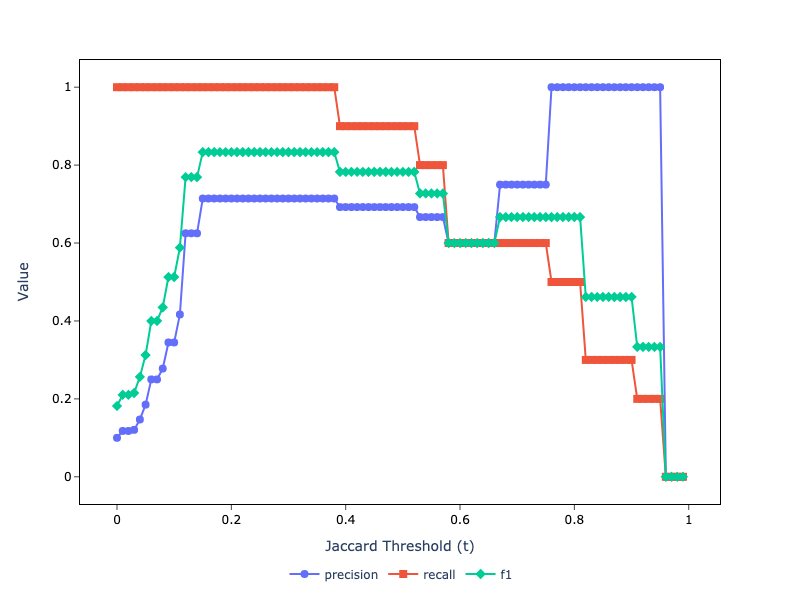
\includegraphics[width=\columnwidth]{mini-buy-fsm-main}
    \caption{Statistical metrics on `mini-buy' dataset
    \textcolor{green}{for results of F-S model}
    }
    \label{fig:mini-buy-fs}
\end{figure}

We can make some observations based on Figure~\ref{fig:mini-buy-fs}.
For values of $t \geq 0.78$, we end up with fewer (lower recall), but more
accurate matches (higher precision) than compared to lower values of $t$ because
the amount of false positives decreases and the amount of false negatives
increases.

For $0.6 \leq t \le 0.78$, precision decreases because the false
positive rate increases and recall increases because the false negative rate
decreases.
This is in line with expectations: the prefix becomes shorter causing a higher
percentage of attributes to be identical.
However, the prefix length is not short enough so that some of the matching
entity references in the ground truth that are more different from one another
will also be captured by \texttt{ppjoin}.

Compared to the previous interval, for values of $0.36 \leq t \le 0.6$, both
precision and recall increase compared to the previous interval.
As the prefix drops, more and more items from the ground truth are matched.
The number of false negatives decreases while the number of false positives
does not increase as fast as the number of true positives.

When $t$ is nearing zero there is an expected increase in recall due to fewer
and fewer overall negatives.
Precision, expectedly decreases due to an ever higher false positive rate.

We need to make a small note on near-identical items in the control data set,
such as \texttt{208114672} and \texttt{208114673}.
For lower values of \textit{t}, the algorithm produces two true positives and
two false positives.
By itself, the increase in false positives intuitively lowers precision.
However, lower values of \textit{t} also broaden the comparison space which
now contains entity references with short values for the name attribute,
like \texttt{205554724}.
By having new items to compare, we also increase the amount of true positives.
This dynamic ends up increasing precision as we lower values of \textit{t} so
long as we are not operating on the full input set.

Note that while we do describe the dynamic specifically for the \texttt{ppjoin}
algorithm, the dynamic of having an increased number of true positives offset
precision in an unexpected direction is not algorithm specific at all.
Regardless of the algorithm that we use, given some circumstances specific for
that algorithm, it should be possible to obtain the same effect we see here.
This observation is interesting because most entity resolution users look at the
F1 score thinking that it provides a good balance between precision and recall.
These users rarely analyse the components of the F1 score.
This situation can lead to unexpected outcomes.
For instance, there might be a substantial drop in F1 scores, which are
indicators of accuracy, when the input data for the entity resolution process is
changed.
The reason for this is that the precision or recall may be higher than expected
for the ideal configuration determined in the controlled scenario.

On the other hand, a balanced trade-off between precision and recall might not
be a requirement.
For instance, a core legal principle applicable in many jurisdictions across the
world states that is far more favourable to let 100 guilty people escape than to
put one innocent behind bars.
By that logic, we only care about precision.
Perfect recall while still retaining some precision might be useful during
research (e.g~finding papers on the same topic) or medical diagnosis (other
cases with the same symptoms).
In these cases, sifting through false positives might be preferable to missing
out on important information because of a false negative that is due to a
suboptimal input configuration.

Our control dataset (which is purposefully flawed) instructs us that the ideal
configuration values for our algorithm are:
\begin{itemize}
    \item $0.15 \leq t \leq 0.38$ for the best balanced outcome
    \item $t \leq 0.38$ for the most sensitive system
    \item $0.76 \leq t \leq 0.95$ for the highest precision
\end{itemize}

\subsubsection{Pairwise Metrics}

The ground truth and the result of the ER process are represented as partitions
over an input set of data.
Because we include the IDs in both DG1 and DG2, the input data set will
contain 20 items.
The ground truth contains 10 pairs of items.

Measuring the similarity of two partitions can be accomplished in more ways than
measuring the statistical success of a matching process.
Among these metrics, the pairwise comparison of two partitions is the best
approximation of the statistical metrics\cite{Men10}.
Figure~\ref{fig:mini-alg-pairwise} shows the computed pairwise metrics for
various values of \textit{t}.

\begin{figure}[!h]
    \centering
    \captionsetup{justification=centering}
    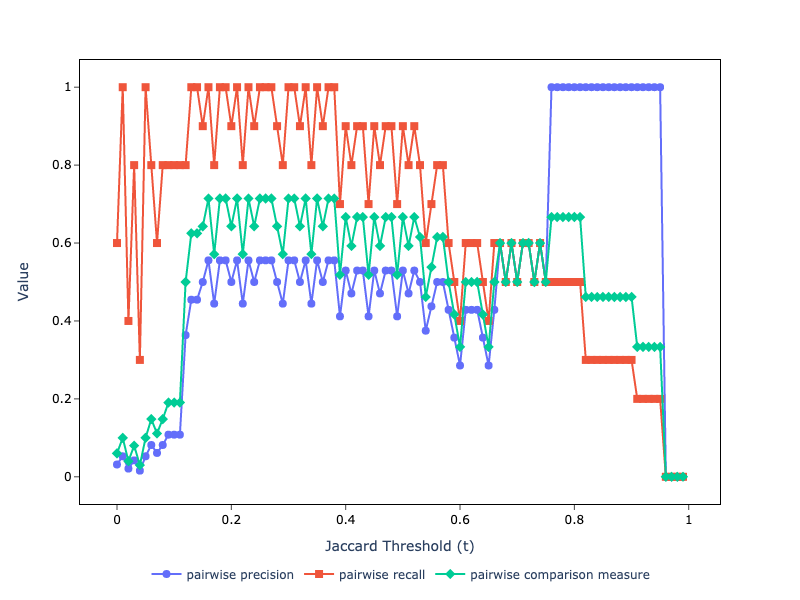
\includegraphics[width=\columnwidth]{mini-buy-algebraic-pairwise}
    \caption{Pairwise metrics on `mini-buy' dataset
    \textcolor{green}{for results of algebric model}\\
    \textcolor{green}{oare in legenda, la verde, nu ar tb sa fie pairwise F1?}
    }
    \label{fig:mini-alg-pairwise}
\end{figure}

We can see a plot similar to the one in Figure~\ref{fig:mini-buy-fs}.
The optimal range for high PF1 scores is the same to the case of statistical measures and the pairwise precision plot's shape
is almost identical (save for a smoother in the statistical model).

It is in terms of recall where we see a major difference from the statistical
model's plot.
More specifically, for $t \le 0.12$ pairwise recall drops significantly whereas
statistical recall stays at the maximum value.
The reason behind this variation lies in the difference between the two models of entity
resolution.
Whereas the standard recall formula only accounts for false negatives (of which
we can not have any using the generated data set), pairwise recall requires the
result data to be partitioned.
The partitioning operation removes any duplicates a partition class might
contain (such as duplicate matches returned by \texttt{ppjoin} for very low
values of \textit{t}).
Probabilistic recall seems to fail to adequately address situations where the
volume of data returned at the end of the entity resolution process vastly
exceeds the size of the ground truth, despite encompassing all true positives.
While in the context of a control dataset this may seem like an unlikely issue,
consider that for practical applications the size of the ground truth is often
several orders of magnitude smaller than the size of the input.

We note again that while the circumstances in which we show this behaviour are
specific to \texttt{ppjoin}, the phenomenon in itself is specific to the model
we employ when we evaluate the algorithm's performance.
Other algorithms may provide the conditions for this phenomenon using their own
input configurations.
To ensure a valid measurement system (one that is both accurate and precise), we
should collect pairwise metrics along with statistical metrics.

\subsubsection{Cluster Metrics}

Pairwise metrics are a form of measuring how well-formed the output of an entity
resolution task is.
The other widely spread family of metrics from this category that resembles
statistical metrics are the cluster metrics, which are displayed in
Figure~\ref{fig:mini-alg-cluster} for 'mini-buy' dataset.

\begin{figure}[!h]
    \centering
    \captionsetup{justification=centering}
    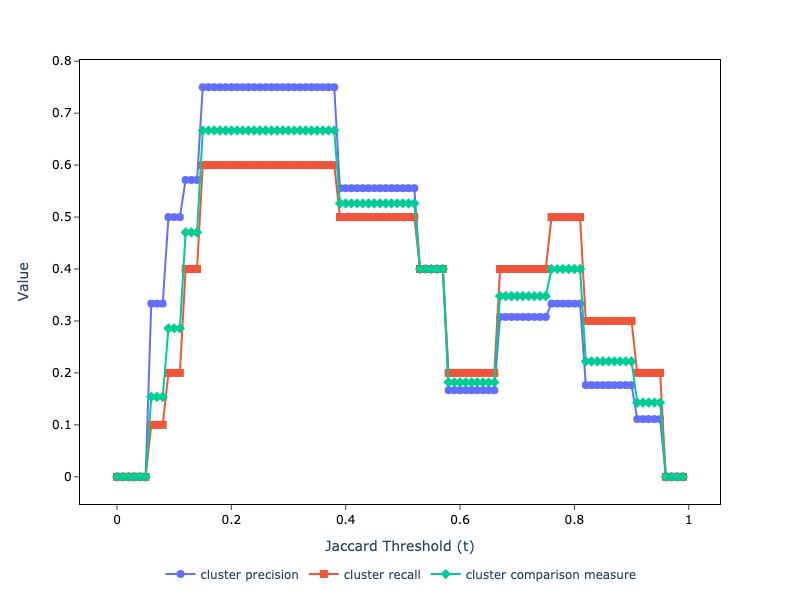
\includegraphics[width=\columnwidth]{mini-buy-algebraic-cluster}
    \caption{Cluster metrics on `mini-buy' dataset 
    \textcolor{green}{for results of algebric model}\\
    \textcolor{green}{oare in legenda, la verde, nu ar tb sa fie cluster F1? (stiu ca e sisnonim cu CCM, dar cand s-a dat formula a fost botezata CF1, iar in prima figura s-a facut referire tot la F1)}
    }
    \label{fig:mini-alg-cluster}
\end{figure}

It is refreshing to see that the optimal value of \textit{t} for a well-balanced
output should still be in the $\left[0.15,0.38\right]$ interval.
We also notice that cluster metrics point out the lack of recall when \textit{t}
nears zero even more than the pairwise metrics.
A more nuanced point is that recall decreases for $t \in \left[0.38,0.58\right]$
much more pronouncedly.

Clustering metrics also reveal interesting aspects about the other metrics we have
seen so far.
For example, we expect increased statistical and pairwise precision to
correspond to increased cluster precision.
This is only somewhat true.
As \textit{t} decreases, we see statistical and pairwise precision increasing
along with cluster precision.
What is interesting is just how much cluster precision increases.
As \textit{t} decreases, more and larger clusters are returned by the entity
resolution task.
For a series of values of \textit{t} the number of returned clusters does not
change much, while the shape of the partition returned by the entity resolution
task becomes more and more similar to the shape of the ground truth.
As the entity resolution task starts returning larger and larger clusters, the
cluster precision drops significantly even though the number of clusters
returned by the entity resolution task drops as well.

A similar effect can be observed for cluster recall as we increase the value of
\textit{t}.
When statistical precision increases, there is a good chance that the number of
clusters in the entity resolution result which are in agreement with the ground
truth would also increase.
Because there are fewer matches as statistical precision increases, we have a
partition that contains many singletons.
This causes cluster precision to decrease (because it relates to the number of
clusters returned by the entity resolution task) and cluster recall to increase
(because it relates to the number of clusters in the ground truth which remains
constant).

These phenomena do not depend on the entity resolution algorithm, but are
characteristics of cluster precision and cluster recall.
Higher statistical recall will always mean fewer and larger clusters some of
which will overlap with clusters in the ground truth.
Higher statistical precision will always mean more singleton clusters returned
by the entity resolution task which, in turn, will increase cluster recall.

Remembering that we might not care about balanced output, we can consider
cluster precision and cluster recall as metrics that balance out the bias built
into statistical precision and recall.
Furthermore, cluster precision and recall can also be used together with
pairwise metrics to confirm any blind spots in the statistical metrics.

In our own practical example, we will use these findings to keep an eye on
$t\in\left[0.76,0.81\right]$ as an interesting input configuration when we are
biased towards better precision.

\subsubsection{Clustering Indexes}

Even though pairwise and cluster metrics complement the statistical metrics,
sometimes all we want is a clear picture of the optimal input configurations for
the algorithm.
The easiest way to glean this information is by using one of the clustering
indexes depicted in Figure~\ref{fig:mini-alg}.

\begin{figure}[!h]
    \centering
    \captionsetup{justification=centering}
    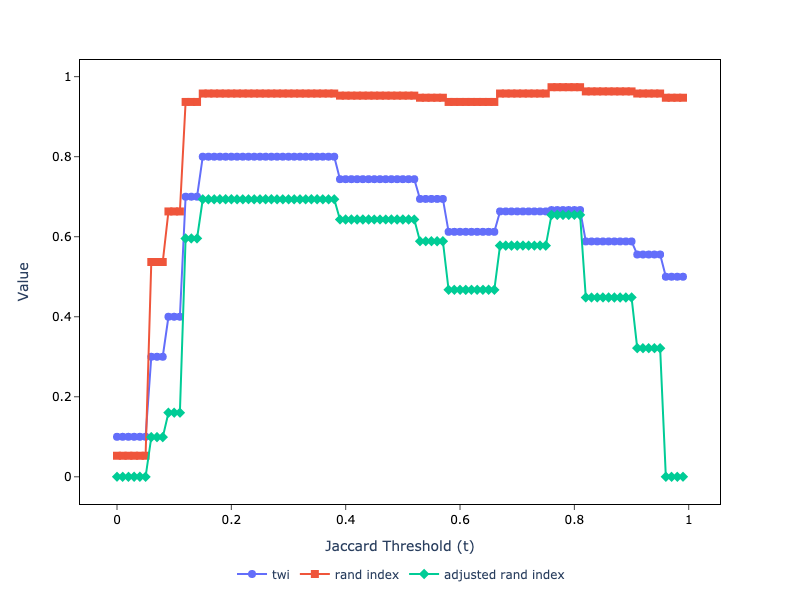
\includegraphics[width=\columnwidth]{mini-buy-algebraic-main}
    \caption{Clustering indexes on `mini-buy' dataset}
    \label{fig:mini-alg}
\end{figure}

We observe that the plot of the Adjusted Rand Index indicates both the desirable
and the undesirable values of \textit{t}.
Notice that it ranks $t\in\left[0.76,0.81\right]$ almost as highly as
$t\in\left[0.15,0.38\right]$.
By following its plot, we should stay clear of values of \textit{t} from other
intervals --- especially those at the extremities of the definition interval.

By comparison with the ARI, the Rand Index itself is not very informative.
It signals that recall is not perfect for values of \textit{t} nearing zero and
does give the highest score for $t\in\left[0.76,0.81\right]$.
However, it also gives high scores for values of \textit{t} where all the other
metrics do not.

The Talburt-Wang index's plot is a fairly good indicator, taking all our former
observations into account.
The only aspect where it is lagging is for $t\in\left[0.76,0.81\right]$.
Here it fails to clarify the favorable circumstances due to high statistical
precision and high cluster recall.

The Adjusted Rand Index or, if operational performance is key, the Talburt-Wang
Index provide enough meaningful information to find ballpark figures for ideal
configuration settings for an entity resolution task.

\subsection{Outcomes from Benchmark Datasets}\label{subsec:experiment-benchmark}

So far we have seen evidence on the generated miniature dataset that each
theoretical model provides a lens through which we can interpret various aspects
of an entity resolution task's qualitative performance.
Some invariants with respect to the entity resolution task have been discovered.
Nothing related to the task that is being evaluated determines these phenomena.
However, we don't know if any of them are invariant with respect to the data
being used.

We want to understand if there are conditions or phenomena that could help us
extract universally good input configurations for an entity resolution algorithm
by using a small dataset.
There already seem to exist some interesting relationships between metrics
including a blind spot in how statistical recall is computed regardless of the
used entity resolution algorithm.
Now we have to see if any of them persist if we change the data used for
performing entity resolution.

In order to do this we shall use benchmark datasets.
The first of these is the `Abt-Buy' data set~\cite{vldb2010} and the plots for
our experiment are available in Figures~\ref{fig:abt-buy-fsm-main},
~\ref{fig:abt-buy-algebraic-pairwise},~\ref{fig:abt-buy-algebraic-cluster}
and~\ref{fig:abt-buy-algebraic-main}.

\begin{figure*}[ht]
    \begin{minipage}{0.24\textwidth}
        \centering
        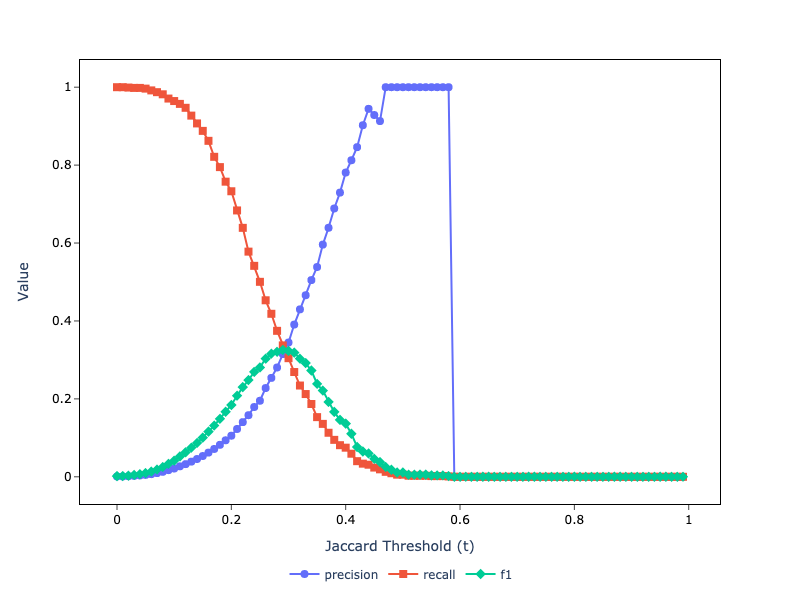
\includegraphics[width=\textwidth]{abt-buy-fsm-main}
        \caption{Abt-Buy statistical metrics.}
        \label{fig:abt-buy-fsm-main}
    \end{minipage}
    \begin{minipage}{0.24\textwidth}
        \centering
        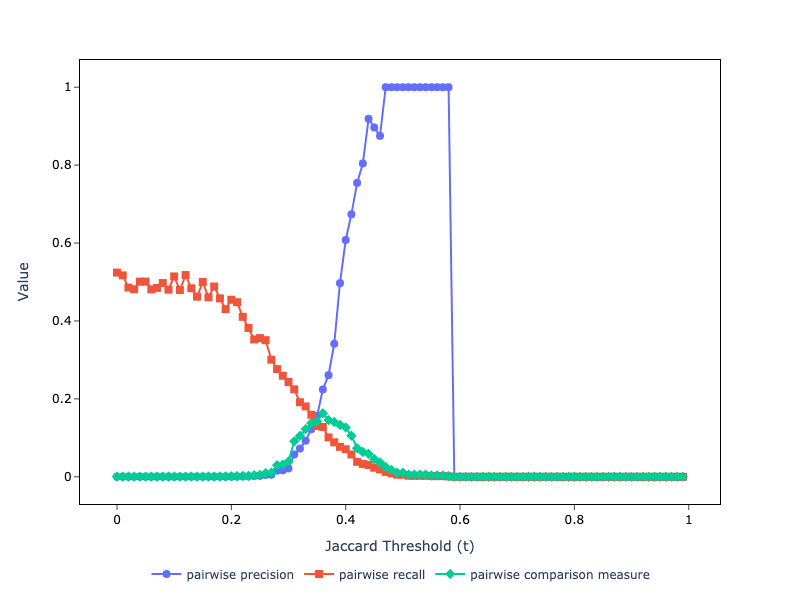
\includegraphics[width=\textwidth]{abt-buy-algebraic-pairwise}
        \caption{Abt-Buy pairwise metrics.}
        \label{fig:abt-buy-algebraic-pairwise}
    \end{minipage}
    \begin{minipage}{0.24\textwidth}
        \centering
        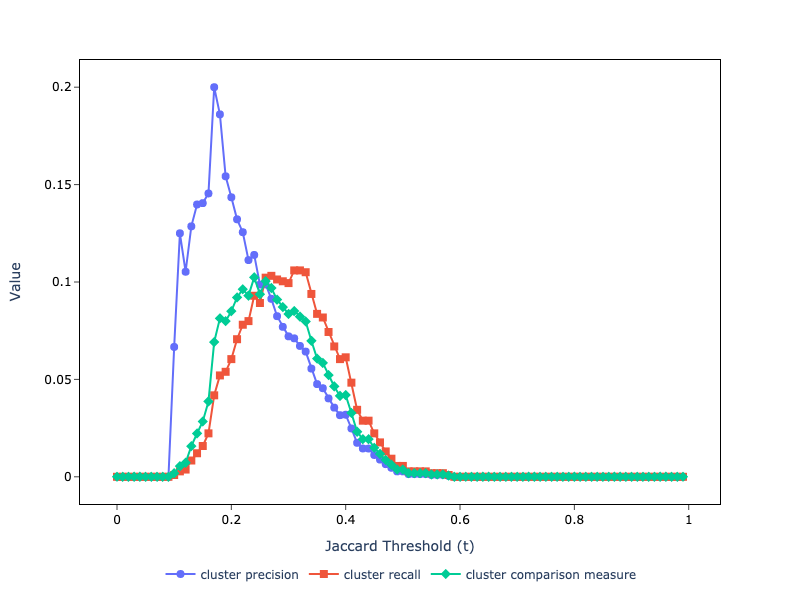
\includegraphics[width=\textwidth]{abt-buy-algebraic-cluster}
        \caption{Abt-Buy cluster metrics.}
        \label{fig:abt-buy-algebraic-cluster}
    \end{minipage}
    \begin{minipage}{0.24\textwidth}
        \centering
        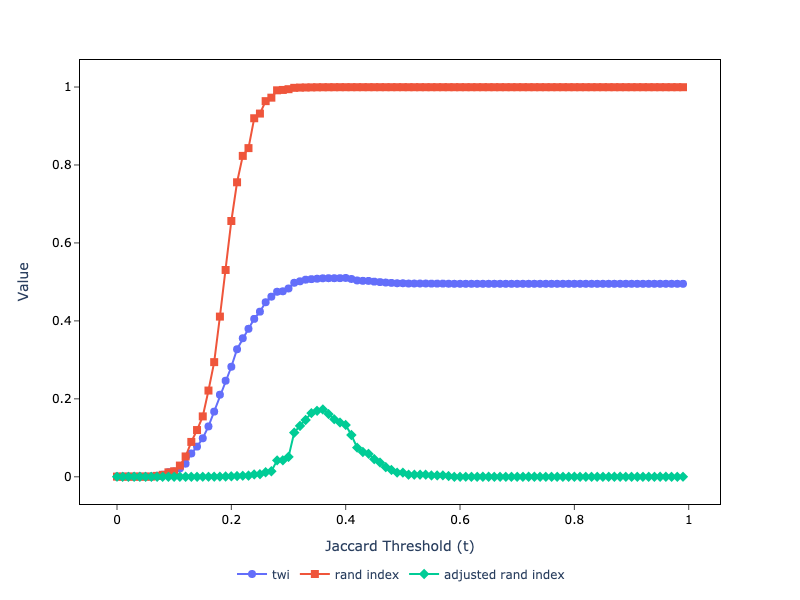
\includegraphics[width=\textwidth]{abt-buy-algebraic-main}
        \caption{Abt-Buy clustering indexes.}
        \label{fig:abt-buy-algebraic-main}
    \end{minipage}
\end{figure*}\label{abt-buy}

We can see that the statistical model still has a pronounced bias towards higher
recall values.
The other invariant that also seems to hold for this dataset as well is the
balancing/confirmation action of the cluster metrics with respect to the
statistical/pairwise metrics.
Another nice confirmation is that the pairwise recall is never perfect.
Lastly, the clustering indexes are good approximates of the ballpark where
we could find  interesting input configurations.
All interesting values of \textit{t} 
\textcolor{green}{I would indicate the value or the value's range for this optimal $t$} 
are in the ballpark indicated by these
indexes.

On the other hand, we can clearly see that input configurations 
\textcolor{green}{la ce anume te referi prin aceste "input configs"? Ai mai amintit si mai devreme, dar nicaieri nu e specifica clar la ce anume se refera; e vorba doar de pagrul $t$ sau si de algoritm de ER si alti params?}  
such as those
that take advantage of a high precision to high cluster recall correlation are
dataset specific.

We move on to the `Amazon-Google Products' data set~\cite{vldb2010} and observe
the results in Figures~\ref{fig:amazon-googleproducts-fsm-main},
\ref{fig:amazon-googleproducts-algebraic-pairwise},
\ref{fig:amazon-googleproducts-algebraic-cluster} and
\ref{fig:amazon-googleproducts-algebraic-main}.

\begin{figure*}[h]
    \begin{minipage}{0.24\textwidth}
        \centering
        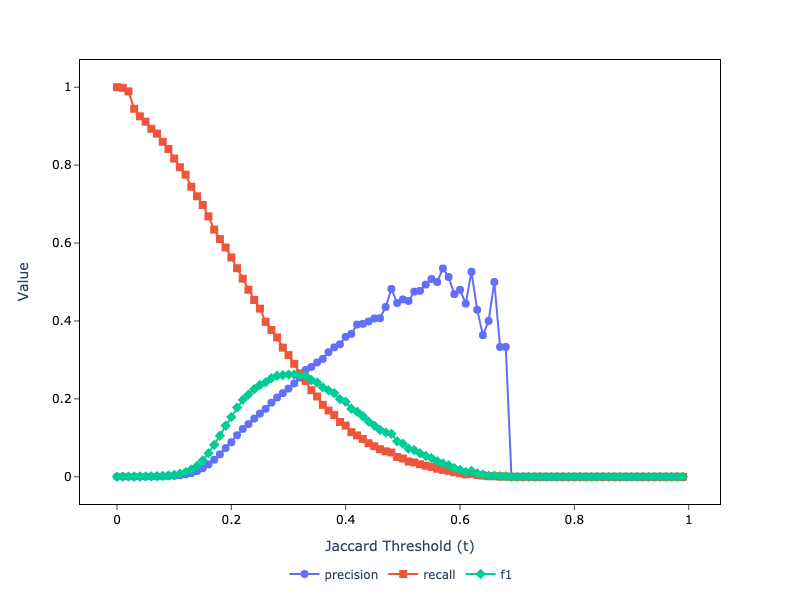
\includegraphics[width=\textwidth]{amazon-googleproducts-fsm-main}
        \caption{Amazon-Google statistical metrics.}
        \label{fig:amazon-googleproducts-fsm-main}
    \end{minipage}
    \begin{minipage}{0.24\textwidth}
        \centering
        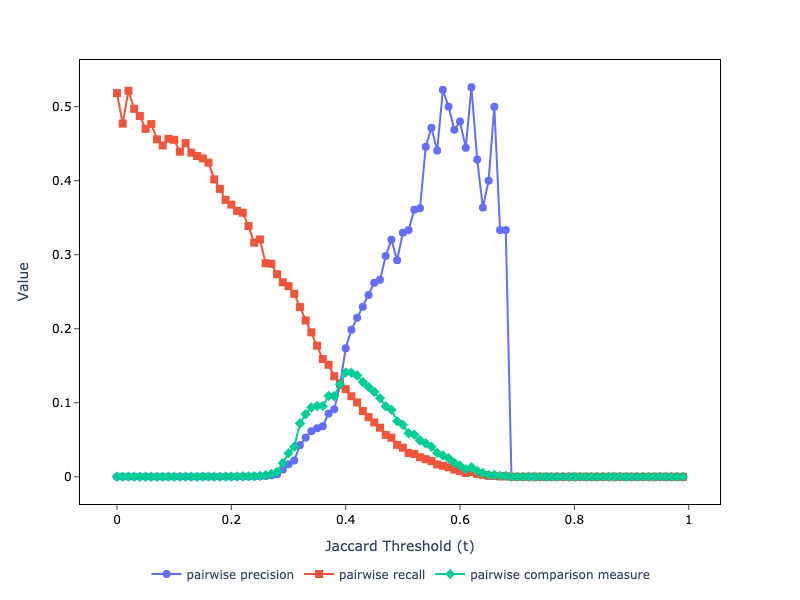
\includegraphics[width=\textwidth]{amazon-googleproducts-algebraic-pairwise}
        \caption{Amazon-Google pairwise metrics.}
        \label{fig:amazon-googleproducts-algebraic-pairwise}
    \end{minipage}
    \begin{minipage}{0.24\textwidth}
        \centering
        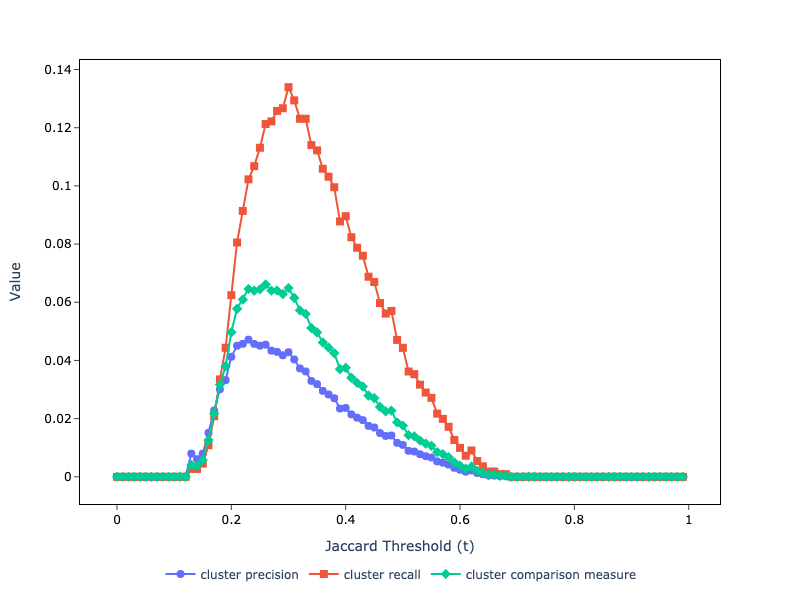
\includegraphics[width=\textwidth]{amazon-googleproducts-algebraic-cluster}
        \caption{Amazon-Google cluster metrics.}
        \label{fig:amazon-googleproducts-algebraic-cluster}
    \end{minipage}
    \begin{minipage}{0.24\textwidth}
        \centering
        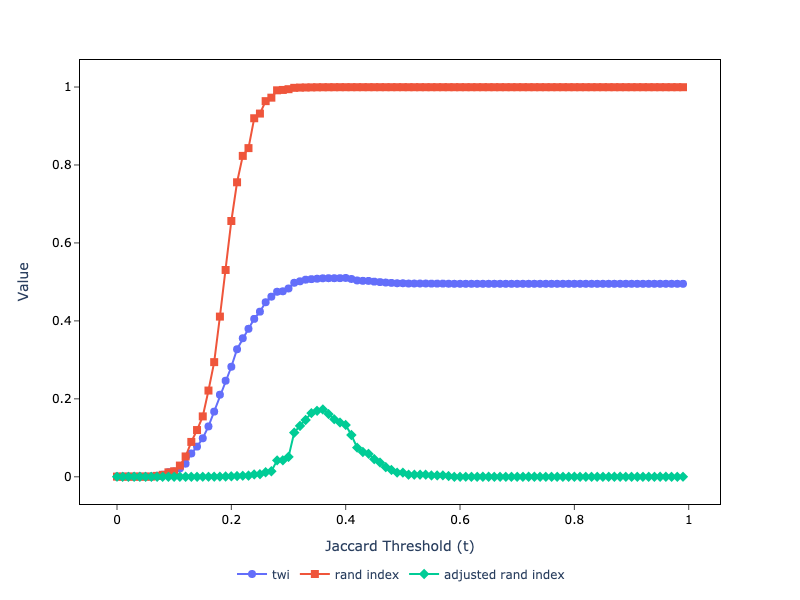
\includegraphics[width=\textwidth]{abt-buy-algebraic-main}
        \caption{Amazon-Google clustering indexes.}
        \label{fig:amazon-googleproducts-algebraic-main}
    \end{minipage}
\end{figure*}\label{amazon-google}

The plotted data shows that the statistical model is biased toward high recall
in this data set, also.
It also shows that pairwise metrics show lower score for recall while
maintaining the shape of the plot for statistical metrics.
Albeit less clearly, we still see that cluster precision and cluster recall can
still act as a balancing weight or confirmation for the statistical metrics or
pairwise metrics, respectively.

On the other hand, we start seeing that the clustering indexes are no longer
individually indicating a ballpark correctly.
The Talburt-Wang index seems to indicate the same optimal input configuration as
the cluster metrics, whereas the Adjusted Rand Index seems to provide a ballpark
of optimal input configurations that would also maximize scores obtained for
pairwise metrics and statistical metrics.
Even though one can assume that this is because of how the two indexes are
defined (TWI counts agreements on whole clusters while ARI counts agreeing
pairs), confirming this assumption experimentally requires further work.
Regardless, we can safely conclude that whether clustering indexes reveal
ballparks for optimal input configurations is dataset dependent.
\textcolor{green}{mie nu mi-e clar ce ai vrut sa spui :(}

Finally, we look at the `DBLP-ACM' benchmark dataset~\cite{vldb2010}.
The plots we obtained after running the experiment on this dataset are available
in Figures~\ref{fig:dblp2-acm-fsm-main},
\ref{fig:dblp2-acm-algebraic-pairwise},
\ref{fig:dblp2-acm-algebraic-cluster} and
\ref{fig:dblp2-acm-algebraic-main}.

\begin{figure*}[h]
    \begin{minipage}{0.24\textwidth}
        \centering
        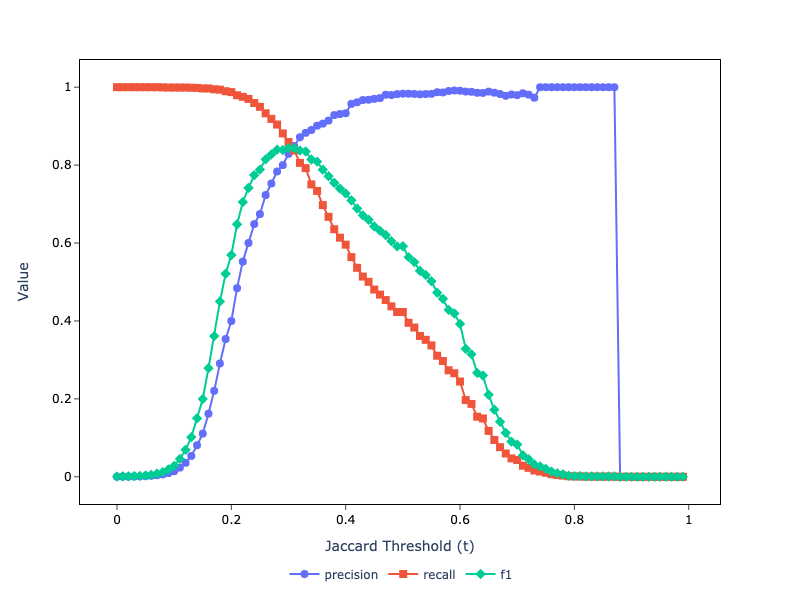
\includegraphics[width=\textwidth]{dblp2-acm-fsm-main}
        \caption{DBLP-ACM statistical metrics.}
        \label{fig:dblp2-acm-fsm-main}
    \end{minipage}
    \begin{minipage}{0.24\textwidth}
        \centering
        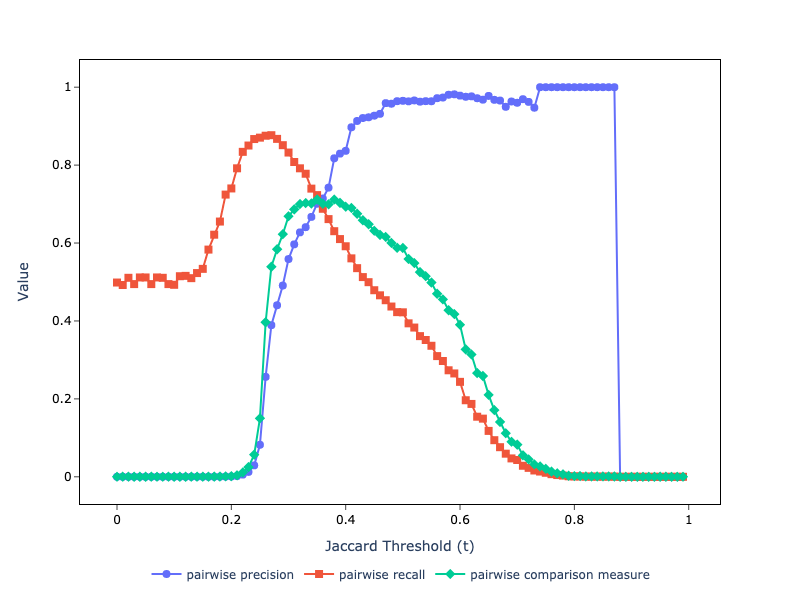
\includegraphics[width=\textwidth]{dblp2-acm-algebraic-pairwise}
        \caption{DBLP-ACM pairwise metrics.}
        \label{fig:dblp2-acm-algebraic-pairwise}
    \end{minipage}
    \begin{minipage}{0.24\textwidth}
        \centering
        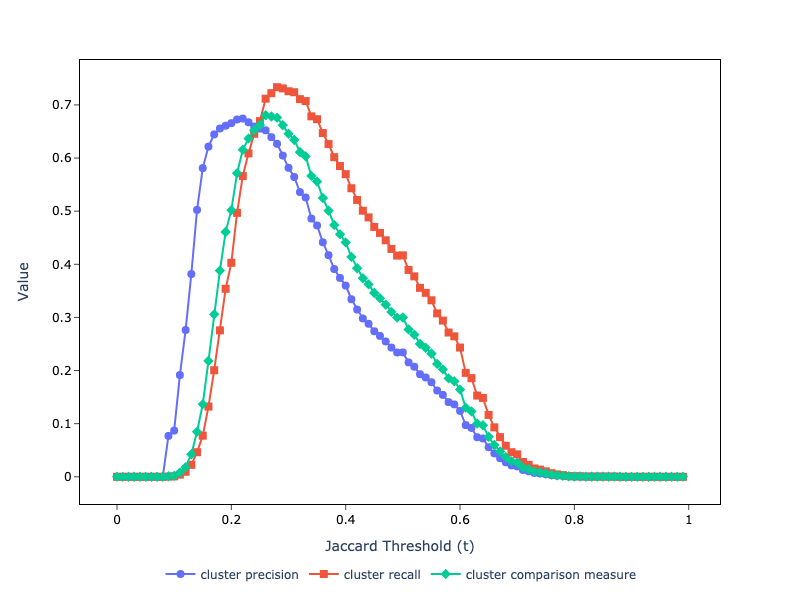
\includegraphics[width=\textwidth]{dblp2-acm-algebraic-cluster}
        \caption{DBLP-ACM cluster metrics.}
        \label{fig:dblp2-acm-algebraic-cluster}
    \end{minipage}
    \begin{minipage}{0.24\textwidth}
        \centering
        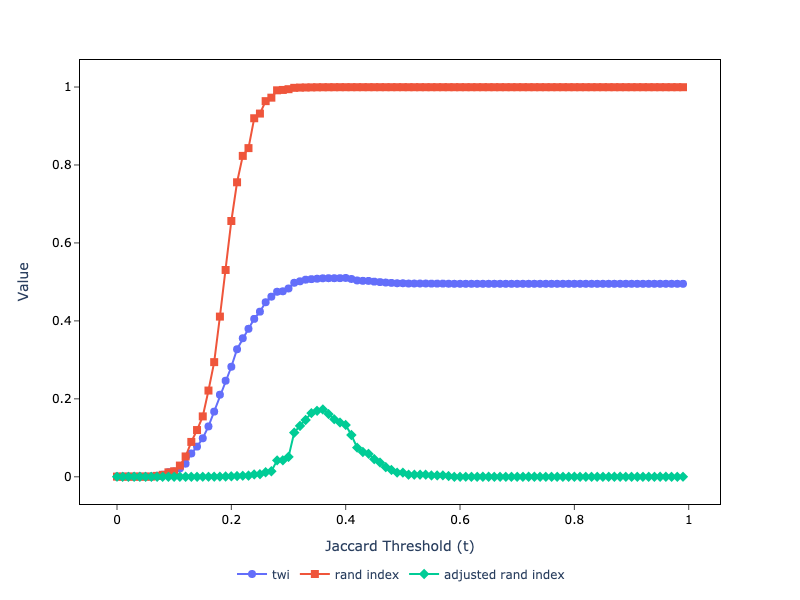
\includegraphics[width=\textwidth]{abt-buy-algebraic-main}
        \caption{DBLP-ACM clustering indexes.}
        \label{fig:dblp2-acm-algebraic-main}
    \end{minipage}
\end{figure*}\label{dblp2-acm}

Looking at the plots for this last dataset we again see confirmation that recall
in the statistical model is much higher than advertised by any of the other
metrics.
The other condition that is invariant with respect to the algorithm and the
data sets is that cluster precision and cluster recall act as good balancing or
confirmation metrics for the statistical and pairwise metrics, respectively.
\textcolor{green}{mie nu mi-e clar ce ai vrut sa spui :(}

We also see that the conjecture concerning the TWI as a good approximation for
input configurations that yield high clustering scores holds for this data set,
too. 
The same can be said about the ARI for approximating high scores with regard to
matching.
These observations hold for all four datasets we have experimented on.


\textcolor{green}{As incerca sa le enunt din nou acest concluzii, iar dupa ce sunt formulate le-as transforma in ipoteze, descriindu-le la inceputul sectiunii cu experimentele; astfel, ele vor reprezenta motivatia: avem 3-4 hipoteze si ne propunem sa le validam prin experimentele efectuate . Eu am retinut asa: \\
1. hypothesis about precision - TBA \\
2. recall in the statistical model is much higher than advertised by any of the other metrics.\\
3. cluster precision and cluster recall act as good balancing or
confirmation metrics for the statistical and pairwise metrics, respectively.\\
4. TWI is a good approximation for input configurations that yield high clustering scores.\\
5. ARI - ???\\
6. ???
}



    \section[conclusion]{Conclusions}\label{sec:conclusions}

    In this paper we have provided an overview of how theoretical models for
    entity resolution influence the data structures that are at play when we are
    working with entity resolution systems in practice.
    The data structures involved using the Fellegi-Sunter model for entity
    resolution revolve around pairs of entity references, whereas those that
    are specific to the algebraic model are centered around sets and partitions
    over sets.
    One interesting finding is that a transition from the Fellegi-Sunter model
    to the algebraic model is possible using the Union-Find data structure and
    a simplified version of Kruskal's algorithm.

    Having this knowledge we ran an experiment using the \texttt{ppjoin}
    algorithm on a generated data set.
    By looking at the results we saw how theoretical models provide different
    perspectives on the same algorithm.
    Having this outlook on things, we were able to glean insights that have
    nothing to do with the algorithm but with the perspectives themselves.

    To see whether the perspectives change if the underlying data changes, we
    ran the experiment on three different benchmark datasets.
    A first conjecture that arises after doing so states that the Fellegi-Sunter
    model for entity resolution provides a perspective over the quality of the
    entity resolution results which is overly optimistic in evaluating recall.
    This leads to higher F1 scores and possibly to wrong conclusions when
    comparing entity resolution solutions using the F1 score.

    The second conjecture is that we can safely use the Talburt-Wang Index to
    find input configurations of the entity resolution task in which it performs
    clustering well.
    The Adjusted Rand Index can be used in the same way to find input conditions
    where the entity resolution task performs matching well.

    We will not draw any conclusion with regard to extrapolating observations on
    smaller sets to larger sets of data or to the overall performance of the
    algorithm even though the data suggests that at least the ballpark stays the
    same.
    In order to make such claims, we need to design and run experiments using
    other entity resolution algorithms.

    \section[future]{Future Work}\label{sec:future}

    In terms of theory, we would like to consider other models for entity
    resolution.
    Firstly, there's existing models such as the one proposed by the Stanford
    Entity Resolution Framework\cite{Ben2009Swoosh} or the graph theoretical
    model of entity resolution which is widely used in entity alignment tasks.
    Then there are theoretical models that we can imagine in the realms of
    recommender systems or a retrieval augmented generative AI.

    The other route to take is to run experiments using more and more algorithms
    to find out whether the conjectures outlined in this paper are worth proving.
    Given the costs of fine-tuning an entity resolution system, a good step
    forward seems to be finding some invariants that would allow us to test
    the system with smaller datasets.

    Lastly, this paper was about finding invariants in the realm of qualitative
    measurements of entity resolution tasks.
    Implementing a system that shows the qualitative and quantitative metrics
    of any entity resolution task would make adopting and tuning entity
    resolution systems less costly and more transparent.

    \bibliographystyle{ieeetr} % We choose the "plain" reference style
    \bibliography{er-general,er-related-work,er-additional-references,er-software}
\end{document}
